% Options for packages loaded elsewhere
\PassOptionsToPackage{unicode}{hyperref}
\PassOptionsToPackage{hyphens}{url}
\PassOptionsToPackage{dvipsnames,svgnames,x11names}{xcolor}
%
\documentclass[
]{article}

\usepackage{amsmath,amssymb}
\usepackage{setspace}
\usepackage{iftex}
\ifPDFTeX
  \usepackage[T1]{fontenc}
  \usepackage[utf8]{inputenc}
  \usepackage{textcomp} % provide euro and other symbols
\else % if luatex or xetex
  \usepackage{unicode-math}
  \defaultfontfeatures{Scale=MatchLowercase}
  \defaultfontfeatures[\rmfamily]{Ligatures=TeX,Scale=1}
\fi
\usepackage{lmodern}
\ifPDFTeX\else  
    % xetex/luatex font selection
\fi
% Use upquote if available, for straight quotes in verbatim environments
\IfFileExists{upquote.sty}{\usepackage{upquote}}{}
\IfFileExists{microtype.sty}{% use microtype if available
  \usepackage[]{microtype}
  \UseMicrotypeSet[protrusion]{basicmath} % disable protrusion for tt fonts
}{}
\makeatletter
\@ifundefined{KOMAClassName}{% if non-KOMA class
  \IfFileExists{parskip.sty}{%
    \usepackage{parskip}
  }{% else
    \setlength{\parindent}{0pt}
    \setlength{\parskip}{6pt plus 2pt minus 1pt}}
}{% if KOMA class
  \KOMAoptions{parskip=half}}
\makeatother
\usepackage{xcolor}
\usepackage[top=2cm,bottom=2cm,left = 2.5cm,right = 2.5cm]{geometry}
\setlength{\emergencystretch}{3em} % prevent overfull lines
\setcounter{secnumdepth}{5}
% Make \paragraph and \subparagraph free-standing
\ifx\paragraph\undefined\else
  \let\oldparagraph\paragraph
  \renewcommand{\paragraph}[1]{\oldparagraph{#1}\mbox{}}
\fi
\ifx\subparagraph\undefined\else
  \let\oldsubparagraph\subparagraph
  \renewcommand{\subparagraph}[1]{\oldsubparagraph{#1}\mbox{}}
\fi


\providecommand{\tightlist}{%
  \setlength{\itemsep}{0pt}\setlength{\parskip}{0pt}}\usepackage{longtable,booktabs,array}
\usepackage{calc} % for calculating minipage widths
% Correct order of tables after \paragraph or \subparagraph
\usepackage{etoolbox}
\makeatletter
\patchcmd\longtable{\par}{\if@noskipsec\mbox{}\fi\par}{}{}
\makeatother
% Allow footnotes in longtable head/foot
\IfFileExists{footnotehyper.sty}{\usepackage{footnotehyper}}{\usepackage{footnote}}
\makesavenoteenv{longtable}
\usepackage{graphicx}
\makeatletter
\def\maxwidth{\ifdim\Gin@nat@width>\linewidth\linewidth\else\Gin@nat@width\fi}
\def\maxheight{\ifdim\Gin@nat@height>\textheight\textheight\else\Gin@nat@height\fi}
\makeatother
% Scale images if necessary, so that they will not overflow the page
% margins by default, and it is still possible to overwrite the defaults
% using explicit options in \includegraphics[width, height, ...]{}
\setkeys{Gin}{width=\maxwidth,height=\maxheight,keepaspectratio}
% Set default figure placement to htbp
\makeatletter
\def\fps@figure{htbp}
\makeatother

\usepackage{stmaryrd}
\usepackage{multicol}
\usepackage{graphicx}
\usepackage{ragged2e}
\usepackage{animate, dsfont, here, xspace}
%\usepackage{tikz}
\usepackage{tikz,pgfplots}
 \pgfplotsset{compat=1.17}
%\includepdf[fitpaper=true, pages=-]{img/pdg.pdf}


\DeclareMathOperator{\e}{e}
\DeclareMathOperator{\Determinant}{det}
\renewcommand{\P}{\mathds{P}} %Apparement \P existe déjà ?
\newcommand\N{\mathds{N}}
\newcommand\Norm{\mathcal{N}}
\newcommand\R{\mathds{R}}
\newcommand\Z{\mathds{Z}}
\newcommand\transp[1]{{#1}^T}
%\newcommand\C{\mathds{C}}
%\newcommand\Z{\mathds{Z}}


\newcommand\1{\mathds{1}}
\newcommand{\E}[2][]{{\mathds{E}}_{#1}
  \def\temp{#2}\ifx\temp\empty
  \else
    \left[#2\right]
  \fi
}
\newcommand{\V}[2][]{{\mathds{V}}_{#1}
  \def\temp{#2}\ifx\temp\empty
  \else
    \left[#2\right]
  \fi
}
\newcommand\ud{\,\mathrm{d}}
\newcommand{\ps}[2]{\left\langle #1 \,,\, #2 \right\rangle}

% blocks
\usepackage{environ}
\usepackage[tikz]{bclogo}

\tikzstyle{titlestyle} =[draw=black!80,fill=black!20, text=black,
 right=10pt, rounded corners]
\mdfdefinestyle{symmaryboxstyle}{
	linecolor=black!80, backgroundcolor = black!5,
	skipabove=\baselineskip, innertopmargin=\baselineskip,
	innerbottommargin=\baselineskip,
	userdefinedwidth=\textwidth,
	middlelinewidth=1.2pt, roundcorner=5pt,
	skipabove={\dimexpr0.5\baselineskip+\topskip\relax},
	frametitleaboveskip=\dimexpr-\ht\strutbox\relax,
	innerlinewidth=0pt,
}
\newcounter{summarybox}
\NewEnviron{summary_box}[2][true]{%
\refstepcounter{summarybox} % on incrémente le compteur
\begin{mdframed}[style=symmaryboxstyle,
nobreak=#1,
frametitle={%
      \tikz[baseline=(current bounding box.east),outer sep=0pt]
      \node[titlestyle,anchor=east]
    {Encadré \thesummarybox{} --- #2};}
]
\vspace{-0.5em}
\BODY
\end{mdframed}
}

\usepackage{amsthm}
%\theoremstyle{remark}
\newtheorem*{remarque}{Remarque}

\usepackage{mathrsfs}
\usepackage{fontawesome5}

%\usepackage[style=authoryear,%,uniquename=false, uniquelist=false,
%maxbibnames=2]{biblatex-chicago}
% \usepackage[options]{natbib}
% \bibliographystyle{chicago}

%\DefineBibliographyStrings{english}{andothers={et\addabbrvspace alii}}
\usepackage[authordate16,backend=biber,maxcitenames=2]{biblatex-chicago}
\usepackage{booktabs}
\usepackage{longtable}
\usepackage{array}
\usepackage{multirow}
\usepackage{wrapfig}
\usepackage{float}
\usepackage{colortbl}
\usepackage{pdflscape}
\usepackage{tabu}
\usepackage{threeparttable}
\usepackage{threeparttablex}
\usepackage[normalem]{ulem}
\usepackage{makecell}
\usepackage{xcolor}
\makeatletter
\@ifpackageloaded{caption}{}{\usepackage{caption}}
\AtBeginDocument{%
\ifdefined\contentsname
  \renewcommand*\contentsname{Table of contents}
\else
  \newcommand\contentsname{Table of contents}
\fi
\ifdefined\listfigurename
  \renewcommand*\listfigurename{List of Figures}
\else
  \newcommand\listfigurename{List of Figures}
\fi
\ifdefined\listtablename
  \renewcommand*\listtablename{List of Tables}
\else
  \newcommand\listtablename{List of Tables}
\fi
\ifdefined\figurename
  \renewcommand*\figurename{Figure}
\else
  \newcommand\figurename{Figure}
\fi
\ifdefined\tablename
  \renewcommand*\tablename{Table}
\else
  \newcommand\tablename{Table}
\fi
}
\@ifpackageloaded{float}{}{\usepackage{float}}
\floatstyle{ruled}
\@ifundefined{c@chapter}{\newfloat{codelisting}{h}{lop}}{\newfloat{codelisting}{h}{lop}[chapter]}
\floatname{codelisting}{Listing}
\newcommand*\listoflistings{\listof{codelisting}{List of Listings}}
\makeatother
\makeatletter
\makeatother
\makeatletter
\@ifpackageloaded{caption}{}{\usepackage{caption}}
\@ifpackageloaded{subcaption}{}{\usepackage{subcaption}}
\makeatother
\ifLuaTeX
\usepackage[bidi=basic]{babel}
\else
\usepackage[bidi=default]{babel}
\fi
\babelprovide[main,import]{british}
% get rid of language-specific shorthands (see #6817):
\let\LanguageShortHands\languageshorthands
\def\languageshorthands#1{}
\ifLuaTeX
  \usepackage{selnolig}  % disable illegal ligatures
\fi
\usepackage[]{biblatex}
\addbibresource{biblio.bib}
\usepackage{bookmark}

\IfFileExists{xurl.sty}{\usepackage{xurl}}{} % add URL line breaks if available
\urlstyle{same} % disable monospaced font for URLs
\hypersetup{
  pdftitle={Improving real-time trend estimates using local parametrisation of polynomial regression filters},
  pdflang={en-GB},
  colorlinks=true,
  linkcolor={blue},
  filecolor={Maroon},
  citecolor={Blue},
  urlcolor={Blue},
  pdfcreator={LaTeX via pandoc}}

\title{Improving real-time trend estimates using local parametrisation
of polynomial regression filters}
\author{}
\date{}

\begin{document}
\maketitle

\setstretch{2}
\section*{Abstract}\label{abstract}
\addcontentsline{toc}{section}{Abstract}

This paper examines and compares real-time estimates of the trend-cycle
component using moving averages constructed with local polynomial
regression. It enables to reproduce Henderson's symmetric and Musgrave's
asymmetric filters used in the X-13ARIMA-SEATS seasonal adjustment
algorithm. This paper proposes two extensions of local polynomial
filters for real-time trend-cycle estimates: first including a
timeliness criterion to minimise the phase shift; second with procedure
for parametrising asymmetric filters locally while they are generally
parametrised globally, which can be suboptimal around turning points. An
empirical comparison, based on simulated and real data, shows that
modelling polynomial trends that are too complex introduces more
revisions without reducing the phase shift, and that local
parametrisation reduces the delay in detecting turning points and
reduces revisions. The results are reproducible and all the methods can
be easily applied using the R package \texttt{rjd3filters}.

Keywords: time series, trend-cycle, seasonal adjustment, turning points,
R statistical software.

JEL Classification: E32, E37.

\section{Introduction}\label{introduction}

Analysis of the economic cycle, and in particular the early detection of
turning points, is a major topic in the analysis of economic outlook. To
achieve this, economic indicators are generally seasonally adjusted.
However, in order to improve their interpretability, it may be necessary
to perform additional smoothing to reduce noise, thereby to analyse the
trend-cycle component. By construction, trend-cycle extraction methods
are closely related to seasonal adjustment methods, since they are
generally applied to seasonally adjusted series.

A moving average, or linear filter, is a statistical method that
consists of applying a rolling weighted mean to a times series: for each
date \(t\) it computes a weighted mean of \(p\) past points and \(q\)
future points where \(p,q\geq0\) depends on the moving average. They are
ubiquitous in business cycle extraction and seasonal adjustment methods.
For example, the X-11 seasonal adjustment method
\autocite{ladiray2011seasonal}, used in X-13ARIMA-SEATS software
\autocite{x13}, uses several moving averages to estimate the main
components of a time series. Symmetric filters are applied to the centre
of the series and for trend-cycle extraction, the most popular symmetric
filter is the \textcite{henderson1916note} moving average, which is used
in the X-11 seasonal adjustment algorithm. However, for real-time
estimates, due to the lack of future observations, all these methods
must rely on asymmetric filters to estimate the most recent points. For
example, for trend-cycle extraction, X-11 uses Henderson's symmetric
filter and \textcite{musgrave1964set}'s asymmetric filters on an
extended series using an ARIMA model. Since the predicted values are
linear combinations of past values, this amounts to applying asymmetric
moving averages at the end of the series. If the classic asymmetric
moving averages have good properties regarding the future revisions
induced by the process (for example \textcite{pierce1980SA} shows
similar performances in terms of revisions of X-11 compared to
theoretically superior procedure based on ARIMA forecast models), they
create, by construction, phase shifts that impact the real-time
estimation of turning points, introducing time delay in the detection.

Using local polynomial regression, \textcite{proietti2008} developed a
general class of symmetric and asymmetric moving averages. In
particular, this class encompass Henderson's symmetric filter and
Musgrave's asymmetric filters. The aim of this study is to propose two
extensions to the \textcite{proietti2008} class of filters in order to
take account of two drawbacks of those methods. Firstly adding, in the
optimisation process, a timeliness criterion to directly control the
phase shift (i.e., the delay in detecting turning points). Secondly
calibrating asymmetric filters locally, while they are generally
calibrated globally using thus assumptions that may be wrong locally.
Those extensions are implemented in the statistical software R
\autocite{logicielr} throw the \texttt{rjd3filters} package
\autocite{rjd3filters} and can therefore be easily used. All the code
associated to this paper is available at \url{https://github.com/XXXX}
(anonymized linked before the manuscript is accepted).

In section~\ref{sec-propMM}, we describe the general properties of
moving averages and the associated quality criteria. This allows us to
understand the foundations behind the construction of moving averages
from local polynomial regressions, as well as those behind the two
extensions proposed in this article (section~\ref{sec-nonparamreg}). In
section~\ref{sec-comparison}, all these methods are compared empirically
on simulated and real series.

\section{Local trend-cycle models and moving averages}\label{sec-propMM}

The basic assumption used in time series decomposition methods is that
the input observed time series, \(y_t\), can be decomposed into a signal
component \(\mu_t\) and an erratic component \(\varepsilon_t\) (called
irregular): \[
f(y_t)=\mu_t+\varepsilon_t
\] where \(f\) denotes some appropriate transformation (usually
logarithmic or no transformation). To simplify further notations,
\(y_t\) will denote the transformed observed series. The noise component
\(\varepsilon_t\) is usually assumed to be a white noise. Assuming that
the input time series is seasonally adjusted (or without seasonality),
the signal \(\mu_t\) represents the trend (sustained and systematic
variations over a long period of time) and cycle (cyclical movements
superimposed upon the long-term trend) components, here estimated
jointly and called trend-cycle \(TC_t\). This component can be locally
approximated by a polynomial degree (section~\ref{sec-nonparamreg}): \[
\mu_t = \sum_{j=0}^d\beta_jt^j+\xi_t
\] with \(\xi_t\) a stochastic process uncorrelated with
\(\varepsilon_t\). Even if some papers model \(\xi_t\) and
\(\varepsilon_t\) separately \autocite[see for
example][]{GrayThomson2002}, a usual assumption, adopted in this paper,
is to is to gather \(\xi_t\) and \(\varepsilon_t\). Thus, the
trend-cycle \(TC_t\) is considered as deterministic and modelled as a
polynomial trend of degree \(d\). The coefficients
\((\beta_0,\dots,\beta_k)\) can be estimated by weighted least squares.
The estimate \(\hat \beta_0\) provides the trend-cycle estimate
\(\widehat{TC}_t\) and it can be shown that this equivalent to apply of
moving average (section~\ref{sec-nonparamreg}). The goal of this paper
is to present two new methods to separate the trend-cycle component from
the noise component in real-time (i.e., when no future point is known),
using moving averages build on local polynomial smoothing techniques.

Numerous papers describe the definition and the properties of moving
averages and linear filters, see for example \textcite{ch12HBSA}. In
this section we summarize some of the main results to understand the
next sections.

Let \(p\) and \(f\) two integers, a moving average
\(M_{\boldsymbol\theta}\) is defined by a set of coefficients
\(\boldsymbol\theta=\transp{\begin{pmatrix}\theta_{-p}&\cdots&\theta_{f}\end{pmatrix}}\)
such as for all time series \(y_t\): \[
M_{\boldsymbol\theta}(y_t)=\sum_{k=-p}^{+f}\theta_kX_{t+k}.
\]

\begin{itemize}
\item
  \(p+f+1\) is called the \emph{moving average order}.
\item
  When \(p=f\) the moving average is said to be \emph{centred}. If we
  also have \(\forall k:\:\theta_{-k} = \theta_k\), the moving average
  \(M_{\boldsymbol\theta}\) is said to be \emph{symmetric}. In this
  case, the quantity \(h=p=f\) is called the \emph{bandwidth}.
\end{itemize}

\subsection{Gain and phase shift functions}\label{subsec:gain-deph}

To interpret the notions of gain and phase shift, it is useful to
illustrate the effects of moving averages on harmonic series
\(y_t=\e^{-i\omega t}\) with \(\omega\in[0,\pi]\). The moving average
\(M_{\boldsymbol\theta}\) transforms \(y_t\) into: \[
Y_t = M_{\boldsymbol\theta}y_t = \sum_{k=-p}^{+f} \theta_k \e^{-i \omega (t+k)}
= \left(\sum_{k=-p}^{+f} \theta_k \e^{-i \omega k}\right)\cdot y_t.
\] The function
\(\Gamma_{\boldsymbol\theta}(\omega)=\sum_{k=-p}^{+f} \theta_k e^{-i \omega k}\)
is called the \emph{transfer function} or \emph{frequency response
function}. The frequency response function can alternatively be defined
as
\(\Gamma_{\boldsymbol\theta}(\omega)=\sum_{k=-p}^{+f} \theta_k e^{i \omega k}\)
or
\(\Gamma_{\boldsymbol\theta}(\omega)=\sum_{k=-p}^{+f} \theta_k e^{2\pi i \omega k}\).
It can be rewritten as: \[
\Gamma_{\boldsymbol\theta}(\omega) = \rho_{\boldsymbol\theta}(\omega)\e^{i\varphi_{\boldsymbol\theta}(\omega)},
\] where
\(\rho_{\boldsymbol\theta}(\omega)=G_{\boldsymbol\theta}(\omega)=\lvert\Gamma_{\boldsymbol\theta}(\omega)\rvert\)
is the \emph{gain} or \emph{amplitude} function and
\(\varphi_{\boldsymbol\theta}(\omega)\) is the \emph{phase shift} or
\emph{time shift} function. We thus have: \begin{align*}
\rho_{\boldsymbol\theta}(\omega) &=\sqrt{\left(\sum_{k=-p}^{+f}\theta_k\cos(\omega k)\right)^2+
\left(\sum_{k=-p}^{+f}\theta_k\sin(\omega k)\right)^2} \\
\tan \varphi_{\boldsymbol\theta}(\omega) &=- \frac{\sum_{k=-p}^{+f}\theta_k\sin(\omega k)}{\sum_{k=-p}^{+f}\theta_k\cos(\omega k)} \text{ if }\sum_{k=-p}^{+f}\theta_k\cos(\omega k) \ne 0 \\
&= 0 \text{ if }\sum_{k=-p}^{+f}\theta_k\cos(\omega k) = 0.
\end{align*} The phase shift is sometimes represented as
\(\phi_{\boldsymbol\theta}(\omega)=\frac{\varphi_{\boldsymbol\theta}(\omega)}{\omega}\)
to measure it in number of periods. For all symmetric moving averages we
have \(\varphi_{\boldsymbol\theta}(\omega)\equiv 0 \;(modulo\;{\pi})\).

To sum up, applying a moving average to a harmonic times series
(\(y_t=\e^{-i\omega t}\)) affects it in in two different ways:

\begin{itemize}
\item
  by multiplying it by an amplitude coefficient
  \(\rho_{\boldsymbol\theta}\left(\omega\right)\) (gain);
\item
  by ``shifting'' it in time by
  \(\varphi_{\boldsymbol\theta}(\omega)/\omega\) which directly affects
  the detection of turning points. When
  \(\varphi_{\boldsymbol\theta}(\omega)/\omega<0\) the time shift is
  negative: the turning point is detected with delay.
\end{itemize}

Fourier decomposition allows us to analyse any time series as a sum of
harmonic series, and each component (trend, cycle, seasonal, irregular)
is associated with a set of frequencies. With \(\omega = 2\pi/s\), the
harmonic series of frequency \(\omega\) represents a series that repeats
itself every \(s\) periods. For example, for a monthly series (\(s=12\)
observations per year), seasonal movements are those that repeat every
year: they are therefore associated with frequencies \(2\pi/12\) (annual
periodicity), \(2\pi/12\times 2=2\pi/6,\dots,2\pi/12\times 5\). In this
paper, we consider that the trend-cycle is associated with frequencies
in the interval \([0, 2\pi/12]\), i.e., movements recurring at least
every 12 months. Even if different frequencies are sometimes used
(e.g.~\([0, 2\pi/36]\) to consider only cycles of at least 36 months),
this has no impact on the results of the study. The other frequencies,
\([2\pi/12, \pi]\) are associated with the irregular component.

Figure~\ref{fig-graphsmusgrave} shows the gain and phase shift function
for the asymmetric Musgrave filter (see section~\ref{sec-lppasymf})
often used for real-time trend-cycle estimation (i.e., when no point in
the future is known). The gain function is greater than 1 on the
frequencies associated with the trend-cycle (\([0, 2\pi/12]\)): this
means that the trend-cycle is well preserved and that short cycles of 1
to 2 years (\([2\pi/24,2\pi/12]\)) are even amplified. At other
frequencies, the gain function is less than 1, but always positive: this
means that the series smoothed by this moving average will always
contain noise, even if it is attenuated. Analysis of the phase shift
shows that the shorter the cycles, the greater the phase shift: this
means that on series smoothed by this moving average, turning points
could be detected at the wrong date.

\begin{figure}[H]

\caption{\label{fig-graphsmusgrave}Coefficients, gain and phase shift
function for the Musgrave filter used in X-11 in real-time (last
estimate) for monthly series when the bandwidth is 6.}

\centering{

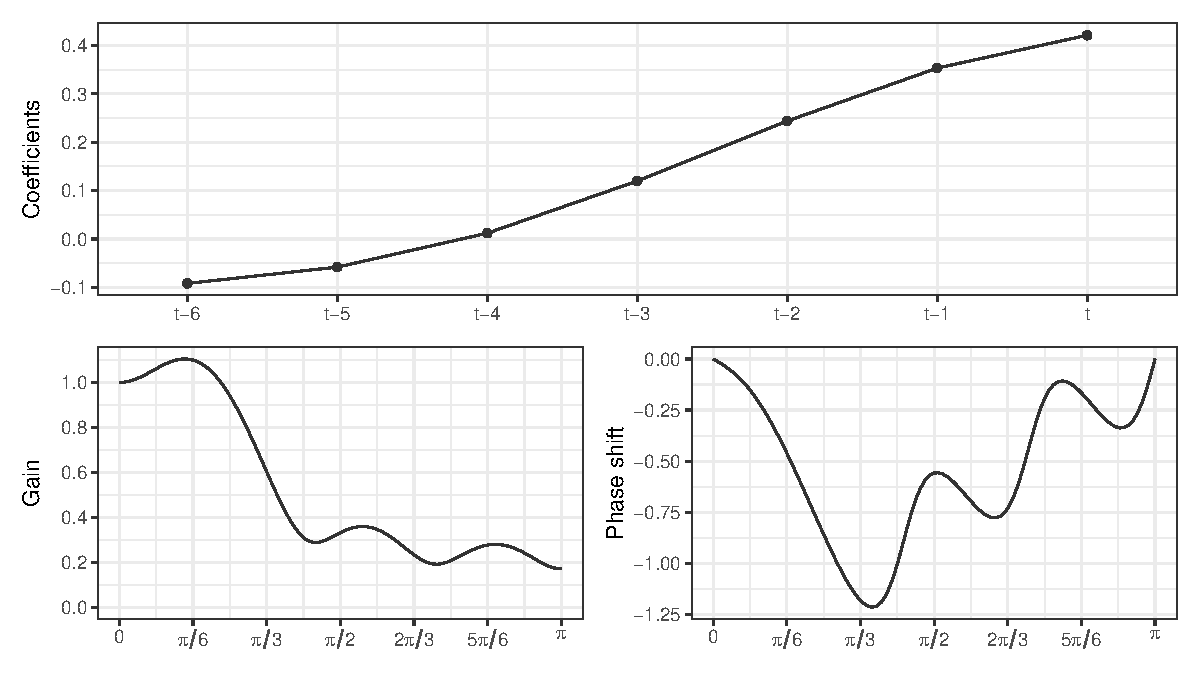
\includegraphics[width=1\textwidth,height=\textheight]{img/filters_used/musgrave.pdf}

\justifying

\emph{Lecture: on monthly times series, 12-month cycles (associated to
the frequency \(2\pi/12=\pi/6\)) are amplified by 10\%
(\(G_{\boldsymbol\theta}(\pi/6)\simeq1.1\)) and associated turning
points are detected with a delay of 1 months
(\(\varphi_{\boldsymbol\theta}(\pi/6)/(\pi/6)\simeq -1\)).}
\emph{8-month cycles (associated to the irregular) are only reduced by
6\% (\(G_{\boldsymbol\theta}(\pi/4)\simeq0.94\)).}\\
\emph{Note: the Musgrave filter depends on a ratio denoted \(I/C\) (see
section~\ref{sec-nonparamreg}).} \emph{In X-11, for monthly series, when
the bandwidth is 6 (i.e.: a symmetric Henderson filter of order 13 is
used, what is used in most cases), the ratio is fixed to 3.5 and this
value is used in this figure.}

}

\end{figure}%

\subsection{Desirable properties of a moving
average}\label{desirable-properties-of-a-moving-average}

To decompose a time series into a seasonal component, a trend-cycle and
the irregular, the X-11 decomposition algorithm (used in
X-13ARIMA-SEATS) uses a succession of moving averages, all with specific
constraints.

In this paper, we assume that our initial series \(y_t\) is seasonally
adjusted and can be written as the sum of a trend-cycle, \(TC_t\), and
an irregular (noise) component, \(\varepsilon_t\): \[
y_t=TC_t+\varepsilon_t.
\] The aim will be to build moving averages that best preserve the
trend-cycle (\(M_{\boldsymbol\theta} (TC_t)\simeq TC_t\)).

Trend-cycles are generally modelled by local polynomial trends (see
section~\ref{sec-nonparamreg}) and, in order to best preserve the
trend-cycles, we thus design moving averages that preserve the
polynomial trends. A moving average \(M_{\boldsymbol\theta}\) preserves
a function of time \(f(t)\) if
\(\forall t,M_{\boldsymbol\theta} f(t)=f(t)\).

For a moving average \(M_{\boldsymbol\theta}\), it can be shown that:

\begin{itemize}
\tightlist
\item
  \(M_{\boldsymbol\theta}\) preserves polynomials of degree \(d\) if and
  only if: \[
  \sum_{k=-p}^{+f}\theta_k=1
   \text{(preserves constant) and }
  \forall j \in \left\{1,2,\dots,d\right\},\:
  \sum_{k=-p}^{+f}k^j\theta_k=0.
  \]
\item
  If \(M_{\boldsymbol\theta}\) is symmetric (\(p=f\) and
  \(\theta_{-k} = \theta_k\)) and preserves polynomials of degree \(2d\)
  then it also preserves polynomials of degree \(2d+1\).
\end{itemize}

\subsection{Real-time estimation and asymmetric moving
average}\label{sec-mmasym}

For symmetric filters, the phase shift function is equal to zero (modulo
\(\pi\)). So there is no delay in detecting turning points. However,
they cannot be used in the beginning and in the end of the time series
because no past or future value can be used. Thus, for real-time
estimation, it is needed to build asymmetric moving averages that
approximate the symmetric moving average.

Several approaches can be used for real-time estimation:

\begin{enumerate}
\def\labelenumi{\arabic{enumi}.}
\item
  Use asymmetric moving averages to take account of the lack of
  available data;
\item
  Apply symmetric filters to an extended forecast series (which is
  equivalent to using asymmetric moving averages, since forecasts are
  linear combinations of the past). This method seems to date back to
  \textcite{deforest1877adjustment}, which also suggests modelling a
  polynomial trend of degree three or less at the end of the period. A
  similar approach is used in the X-13ARIMA-SEATS seasonal adjustment
  method: the series is extended by one year (by default) with an ARIMA
  model to minimise the revisions associated to asymmetric filters.
  Since the final filter used for the seasonal adjustment extraction is
  much longer than one year (in most of the cases, for monthly series,
  the bandwidth is 78), the input series is just partially extended (and
  asymmetric filters are still used) to prevent from instability over
  long periods (e.g., outliers or model shifts).
\end{enumerate}

Conversely, the \emph{implicit forecasts} of an asymmetric moving
average can be deduced from a reference symmetric moving average. This
allows us to judge the quality of real-time estimates of the trend-cycle
and to anticipate future revisions when forecasts are far from expected
evolutions.\\
Let us denote \(\boldsymbol v=(v_{-h},\dots, v_{h})\) the reference
symmetric moving average (used to compute the final estimates) and
\(\boldsymbol w^0,\dots, \boldsymbol w^{h-1}\) a sequence of asymmetric
moving averages used for the intermediate estimates.
\(\boldsymbol w^0=(w_{-h}^0, \dots, w_{0}^0)\) is used for estimation in
real-time estimate (when 0 point in the future is known),
\(\boldsymbol w^1=(w_{-h}^1, \dots, w_{0}^1, w_{1}^1)\) is used for
estimation of the penultimate point (when only 1 in the future is
known), and so on. Let \(y_{t-h},\dots,y_{t}\) be the observed series
during the last \(h\) periods (for which asymmetric moving averages are
used to get the intermediate trend-cycle estimates for the dates \(t-h\)
to \(t\)). The \emph{implicit forecast} \(y_{t+1}^*,\dots y_{t+h}^*\)
induced by \(w^0,\dots w^{h-1}\) are the forecasts of the series \(y_t\)
for which the estimates of the symmetric filter applied to the extended
series
\(\boldsymbol y^* = (y_{t-h}, \dots, y_t, y_{t+1}^*,\dots y_{t+h}^*)\)
produce the same estimates as the asymmetric filter applied to the
series \(\boldsymbol y^*\). This means: \begin{align*}
\underbrace{\sum_{i=-h}^0 v_iy_{t+i} + \sum_{i=1}^h v_iy_{t+i}^*}_{\text{smoothing by }\boldsymbol v\text{ of the extended series}} &=
\underbrace{\sum_{i=-h}^0 w_i^0y_{t+i}}_{\text{smoothing by }\boldsymbol w^0\text{ using }0\text{ point after }t} \\
&=
\underbrace{\sum_{i=-h}^0 w_i^1y_{t+i} + w_1^1y_{t+1}^*}_{\text{smoothing by }\boldsymbol w^1\text{ using }1\text{ point after }t} \\
&= \underbrace{\sum_{i=-h}^0 w_i^2y_{t+i} + \sum_{i=1}^{2}w_i^2y_{t+i}^*}_{\text{smoothing by }\boldsymbol w^2\text{ using }2\text{ points after }t} \\
&= \cdots \\
&=\underbrace{\sum_{i=-h}^0 w_i^{h-1}y_{t+i} + \sum_{i=1}^{h-1} w_i^{h-1}y_{t+i}^*}_{\text{smoothing by }\boldsymbol w^{h-1}\text{ using }h-1\text{ points after }t}
\end{align*} For any integer \(q\) between 0 and \(h-1\), using for
convention \(w_t^q=0\) if \(t>q\) we then have: \[
\sum_{i=1}^h (v_i- w_i^q) y_i^*
=\sum_{i=-h}^0 (w_i^q-v_i)y_i.
\] In matrix form, this is equivalent to solving: \[
\scriptstyle
\begin{pmatrix}
  v_1 & v_2 & \cdots & v_h \\
  v_1 - w_1^1 & v_2 & \cdots & v_h \\
  \vdots & \vdots & \cdots & \vdots \\
   v_1 - w_1^{h-1} & v_2-w_2^{h-1} & \cdots & v_h
\end{pmatrix}
\begin{pmatrix}y_1^* \\ \vdots \\ y_h^*\end{pmatrix}=
\begin{pmatrix}
  w_{-h}^0 - v_{-h} & w_{-(h-1)}^0 - v_{-(h-1)} & \cdots & w_{0}^0 - v_{0} \\
  w_{-h}^1 - v_{-h} & w_{-(h-1)}^1 - v_{-(h-1)} & \cdots & w_{0}^1 - v_{0} \\
  \vdots & \vdots & \cdots & \vdots \\
  w_{-h}^{h-1} - v_{-h} & w_{-(h-1)}^{h-1} - v_{-(h-1)} & \cdots & w_{0}^{h-1} - v_{0}
\end{pmatrix}
\begin{pmatrix}y_{-h} \\ \vdots \\ y_0\end{pmatrix}.
\] This is implemented in the \texttt{rjd3filters::implicit\_forecast()}
function.

As highlighted by \textcite{wildischis2004}, extending the series
through forecasting with an ARIMA model is equivalent to calculating
asymmetric filters whose coefficients are optimised in relation to the
one-step ahead forecast. In other words, the aim is to minimise the
revisions between the first and last estimates (with the symmetric
filter). However, the phase shift induced by the asymmetric filters is
not controlled: we might prefer to have faster detection of turning
points and a larger revision rather than just minimising the revisions
between the first and last estimates. Furthermore, since the
coefficients of the symmetric filter (and therefore the weight
associated with distant forecasts) decrease slowly, we should also be
interested in the performance of multi-step ahead forecasting. This is
why it may be necessary to define alternative criteria for judging the
quality of asymmetric moving averages.

\section{Non-parametric regression and local polynomial
regression}\label{sec-nonparamreg}

Many trend-cycle extraction methods are based on non-parametric
regressions, which are particularly flexible because they do not assume
any predetermined dependency in the predictors. In practice, local
regressions can be used. More specifically, consider a set of points
\((x_t,y_t)_{1\leq t\leq n}\) and we here consider that \(x_t=t\) (no
external regressor is used). Non-parametric regression involves assuming
that there exists a function \(\mu\), to be estimated, such that
\(y_t=\mu(t)+\varepsilon_t\) with \(\varepsilon_t\) an error term.
According to Taylor's theorem, for any date \(t_0\), if \(\mu\) is
differentiable \(d\) times, then:
\begin{equation}\phantomsection\label{eq-taylor}{
\forall t,\:\mu(t) = \underbrace{\mu(t_0)}_{=TC_{t_0}} + \mu'(t_0)(t-t_0)+\dots +
\frac{\mu^{(d)}(t_0)}{d!}(t-t_0)^d+R_d(t),
}\end{equation} where \(R_d\) is a negligible residual term in the
neighbourhood of \(t_0\). In a neighbourhood \(h(t_0)\) around \(t_0\),
\(\mu\) can therefore be approximated by a polynomial of degree \(d\).
The quantity \(h(t_0)\) is called the \emph{bandwidth}. If
\(\varepsilon_t\) is white noise, we can estimate \(\mu(t_0)=TC_{t_0}\)
by least squares using the observations which are in
\(\left[t_0-h(t_0),t_0+h(t_0)\right]\). In practice, this means assuming
that the trend is locally polynomial. We also generally assume that the
bandwidth is fixed over time: \(h(t_0)=h.\) This is also what is assumed
in the seasonal adjustment algorithm X-11 and what will be assumed in
this paper.

Various estimation methods can be used to derive symmetric and
asymmetric moving averages. For example, \textcite{GrayThomson1996}
propose a complete statistical framework that makes it possible, in
particular, to model the error in approximating the trend by local
polynomials. However, as the specification of this error is generally
complex, simpler models may be preferred, such as that of
\textcite{proietti2008}. \textcite{dagumbianconcini2008} propose a
similar modelling of the trend-cycle but using the theory of Hilbert
spaces with reproducing kernels for estimation, which has the particular
advantage of facilitating the calculation of different moving averages
at different time frequencies. See \textcite{inseeDTM202401} for a more
detailed comparison of the different recent methods for trend-cycle
extraction included in the \texttt{rjd3filters} package.

In this paper we will focus on \textcite{proietti2008} approach.
Section~\ref{sec-sym-lp} and section~\ref{sec-lppasymf} describes their
approach to build symmetric moving averages (used for the final
estimates of the trend-cycle component) and asymmetric moving averages
(used for real-time estimates). This paper proposed two extensions of
their approach to build asymmetric moving averages: a first one adding a
criteria to control the phase shift (section~\ref{sec-localic}), not
used in the simulation (section~\ref{sec-comparison}) but which could be
used in future studied; a second one using a local parametrisation of a
parameter usually parametrised globally
(section~\ref{sec-lptimeliness}), which is used in the simulation.

\subsection{Symmetric moving averages and local polynomial
regression}\label{sec-sym-lp}

Using \textcite{proietti2008}'s framework, we assume that our time
series \(y_t\) can be decomposed into \[
y_t=TC_t+\varepsilon_t,
\] where \(TC_t\) is the trend-cycle and
\(\varepsilon_{t}\overset{i.i.d}{\sim}\mathcal{N}(0,\sigma^{2})\) is the
noise (the series is therefore seasonally adjusted). Within a
neighbourhood \(h\) of \(t\), the local trend \(TC_t\) is approximated
by a polynomial of degree \(d\), such that \(TC_t\simeq m_{t}\) with: \[
\forall j\in\left\{-h,-h+1,\dots,h\right\},\:
y_{t+j}=m_{t+j}+\varepsilon_{t+j},\quad m_{t+j}=\sum_{i=0}^{d}\beta_{i}j^{i}.
\] The problem of trend extraction is equivalent to estimating
\(m_t=TC_t=\beta_0\) (the constant in the previous formula).

In matrix notation: \begin{equation}\phantomsection\label{eq-lpp}{
\underbrace{\begin{pmatrix}y_{t-h}\\
y_{t-(h-1)}\\
\vdots\\
y_{t}\\
\vdots\\
y_{t+(h-1)}\\
y_{t+h}
\end{pmatrix}}_{\boldsymbol y}=\underbrace{\begin{pmatrix}1 & -h & h^{2} & \cdots & (-h)^{d}\\
1 & -(h-1) & (h-1)^{2} & \cdots & (-(h-1))^{d}\\
\vdots & \vdots & \vdots & \cdots & \vdots\\
1 & 0 & 0 & \cdots & 0\\
\vdots & \vdots & \vdots & \cdots & \vdots\\
1 & h-1 & (h-1)^{2} & \cdots & (h-1)^{d}\\
1 & h & h^{2} & \cdots & h^{d}
\end{pmatrix}}_{\boldsymbol X}\underbrace{\begin{pmatrix}\beta_{0}\\
\beta_{1}\\
\vdots\\
\vdots\\
\vdots\\
\vdots\\
\beta_{d}
\end{pmatrix}}_{\boldsymbol \beta}+\underbrace{\begin{pmatrix}\varepsilon_{t-h}\\
\varepsilon_{t-(h-1)}\\
\vdots\\
\varepsilon_{t}\\
\vdots\\
\varepsilon_{t+(h-1)}\\
\varepsilon_{t+h}
\end{pmatrix}}_{\boldsymbol \varepsilon}.
}\end{equation}

Since \(d+1\) parameters are estimated with \(\boldsymbol \beta\), we
need at least \(2h+1\) observations (thus \(2h\geq d\)) and the
estimation is made by weighted least squares (WLS), which is equivalent
to minimising the following objective function: \[
S(\hat{\beta}_{0},\dots,\hat{\beta}_{d})=\sum_{j=-h}^{h}\kappa_{j}(y_{t+j}-\hat{\beta}_{0}-\hat{\beta}_{1}j-\dots-\hat{\beta}_{d}j^{d})^{2}.
\] where \(\kappa_j\) is a set of weights called a \emph{kernel}. We
have \(\kappa_j\geq 0:\kappa_{-j}=\kappa_j\), and with
\(\boldsymbol K=diag(\kappa_{-h},\dots,\kappa_{h})\), the estimate of
\(\boldsymbol \beta\) can be written as
\(\hat{\boldsymbol\beta}=(\transp{\boldsymbol X}\boldsymbol K\boldsymbol X)^{-1}\transp{\boldsymbol X}\boldsymbol K\boldsymbol y.\)
With
\(\boldsymbol e_1=\transp{\begin{pmatrix}1 &0 &\cdots&0 \end{pmatrix}}\),
the estimate of the trend is:
\begin{equation}\phantomsection\label{eq-mmsym}{
\hat{m}_{t}=\widehat{TC}_t=\boldsymbol e_{1}\hat{\boldsymbol \beta}=\transp{\boldsymbol \theta}\boldsymbol y=\sum_{j=-h}^{h}\theta_{j}y_{t-j}\text{ with }\boldsymbol \theta=\boldsymbol K\boldsymbol X(\transp{\boldsymbol X}\boldsymbol K\boldsymbol X)^{-1}\boldsymbol e_{1}.
}\end{equation} To conclude, the estimate of the trend
\(\widehat{TC}_{t}\) can be obtained applying the symmetric filter
\(\boldsymbol \theta\) to \(y_t\) (\(\boldsymbol \theta\) is symmetric
due to the symmetry of the kernel weights \(\kappa_j\)). Moreover, since
\(\transp{\boldsymbol X}\boldsymbol \theta=\boldsymbol e_{1}\) we have:
\[
\sum_{j=-h}^{h}\theta_{j}=1,\quad\forall r\in\left\{1,2,\dots,d\right\}:\sum_{j=-h}^{h}j^{r}\theta_{j}=0.
\] Hence, the filter \(\boldsymbol w\) preserves deterministic
polynomials of order \(d\).

Regarding parameter selection, the general consensus is that the choice
between different kernels is not crucial. See, for example,
\textcite{cleveland1996smoothing} or \textcite{Loader1999}. The only
desired constraints on the kernel are that it assigns greater weight to
the central estimation (\(\kappa_0\)) and decreases towards 0 as it
moves away from the central observation. The uniform kernel should
therefore be avoided. It is then preferable to focus on two other
parameters:

\begin{itemize}
\item
  the degree of the polynomial, denoted by \(d\): if it is too small,
  there is a risk of biased estimates of the trend-cycle, and if it is
  too large, there is a risk of excessive variance in the estimates (due
  to over-adjustment);
\item
  the number of neighbours \(2h+1\) (or the window \(h\)): if it is too
  small, then there will be too little data for the estimates (resulting
  in high variance in the estimates), and if it is too large, the
  polynomial approximation will probably be wrong, leading to biased
  estimates.
\end{itemize}

In this paper we will use the Henderson kernel: \[
\kappa_{j}=\left[1-\frac{j^2}{(h+1)^2}\right]
\left[1-\frac{j^2}{(h+2)^2}\right]
\left[1-\frac{j^2}{(h+3)^2}\right].
\] However, several other kernels are available in \texttt{rjd3filters}.

\subsection{Asymmetric moving averages and local polynomial
regression}\label{sec-lppasymf}

As mentioned in section~\ref{sec-mmasym}, for real-time estimation,
several approaches can be used:

\begin{enumerate}
\def\labelenumi{\arabic{enumi}.}
\item
  Apply symmetric filters to the series extended by forecasting
  \(\hat{y}_{n+l\mid n},l\in\left\{1,2,\dots,h\right\}\).
\item
  Build an asymmetric filter by local polynomial approximation on the
  available observations (\(y_{t}\) for
  \(t\in\left\{n-h,n-h+1,\dots,n\right\}\)).
\item
  Build asymmetric filters that minimise the mean squared error of
  revision under polynomial trend reproduction constraints.
\end{enumerate}

\textcite{proietti2008} show that the first two approaches are
equivalent when forecasts are made by polynomial extrapolation of degree
\(d\). They are also equivalent to the third approach under the same
constraints as those of the symmetric filter. The third method is called
\emph{direct asymmetric filtering} (DAF). This method is used for
real-time estimation in the STL seasonal adjustment method
(\emph{Seasonal-Trend decomposition based on Loess}, see
\textcite{cleveland90}). Although DAF filter estimates are unbiased,
this is at the cost of greater variance in the estimates.

To solve the problem of the variance of real-time filter estimates,
\textcite{proietti2008} propose a general method for constructing
asymmetric filters that allows a bias-variance trade-off. This is a
generalisation of \textcite{musgrave1964set}'s asymmetric filters (used
in the X-11 seasonal adjustment algorithm).

Rewriting equation~\ref{eq-lpp}:
\begin{equation}\phantomsection\label{eq-lpgeneralmodel}{
\boldsymbol y=\begin{pmatrix}\boldsymbol U &\boldsymbol Z\end{pmatrix}
\begin{pmatrix}\boldsymbol \gamma \\ \boldsymbol \delta\end{pmatrix}+\boldsymbol \varepsilon,\quad
\boldsymbol \varepsilon\sim\mathcal{N}(0,\boldsymbol D).
}\end{equation} where \([\boldsymbol U,\boldsymbol Z]\) is of full rank
and forms a subset of the columns of \(X.\) Defining the variance error
as \(\boldsymbol D = \sigma^2\boldsymbol K^{-1}\) (to directly take into
account the weights associated to the observations) and with
\([\boldsymbol U,\boldsymbol Z] = \boldsymbol X\) we thus find the model
associated to symmetric filters. The objective is to find an asymmetric
filter \(\boldsymbol v\) which uses \(q\) points in the future and
minimises the mean square error of revision (to the symmetric filter
\(\boldsymbol \theta\)) under certain (polynomial) constraints. The
matrices \(\boldsymbol y\), \(\boldsymbol U\), \(\boldsymbol Z\) and
\(\boldsymbol \theta\) are partitioned as follows: \[
\boldsymbol y = \begin{pmatrix} \boldsymbol y_p \\ \boldsymbol y_f \end{pmatrix}, \quad
\boldsymbol U = \begin{pmatrix} \boldsymbol U_p \\ \boldsymbol U_f \end{pmatrix}, \quad  
\boldsymbol Z = \begin{pmatrix} \boldsymbol Z_p \\ \boldsymbol Z_f \end{pmatrix}, \quad 
\boldsymbol \theta = \begin{pmatrix} \boldsymbol \theta_p \\ \boldsymbol \theta_f \end{pmatrix},
\] where \(\boldsymbol y_p\) is a matrix \((h+q+1)\times 1\) which
denotes the set of available observations (from \(y_{t-h}\) to
\(y_{t+q}\)) and \(\boldsymbol U\), \(\boldsymbol Z\) and
\(\boldsymbol \theta\) are partitioned in the same way. The constraints
are defined as
\(\transp{\boldsymbol U_p}\boldsymbol v=\transp{\boldsymbol U}\boldsymbol \theta\):
they represent the polynomial preservation constraints we want to impose
on the asymmetric filter. \(\boldsymbol Z\) is then associated to the
polynomial constraints of the symmetric filter not imposed on asymmetric
filter. \textcite{proietti2008} show that the problem is equivalent to
finding \(v\) which minimises:
\begin{equation}\phantomsection\label{eq-lppasym}{
\varphi(\boldsymbol v)=
\underbrace{
  \underbrace{\transp{(\boldsymbol v-\boldsymbol \theta_{p})}\boldsymbol D_{p}(\boldsymbol v-\boldsymbol \theta_{p})+
  \transp{\boldsymbol \theta_{f}}\boldsymbol D_{f}\boldsymbol \theta_{f}}_\text{revision error variance}+
  \underbrace{[\transp{\boldsymbol \delta}(\transp{\boldsymbol Z_{p}}\boldsymbol v-\transp{\boldsymbol Z}\boldsymbol \theta)]^{2}}_{bias^2}
}_\text{mean square revision error}+
\underbrace{2\transp{\boldsymbol l}(\transp{\boldsymbol U_{p}}\boldsymbol v-\transp{\boldsymbol U}\boldsymbol \theta)}_{\text{constraints}}.
}\end{equation} where \(\boldsymbol l\) is a vector of Lagrange
multipliers.

When \(\boldsymbol U=\boldsymbol X\) (and then
\(\boldsymbol Z = \boldsymbol 0\)), the constraint is equivalent to
preserving polynomials of degree \(d\) and we find asymmetric direct
filters (DAF) when \(\boldsymbol D=\sigma^2\boldsymbol K^{-1}\).

When \(\boldsymbol U=\transp{\begin{pmatrix}1&\cdots&1\end{pmatrix}}\),
\(\boldsymbol Z=\transp{\begin{pmatrix}-h&\cdots&+h\end{pmatrix}}\),
\(\boldsymbol \delta=\delta_1\), \(\boldsymbol D=\sigma^2\boldsymbol I\)
and when the symmetric filter is the Henderson filter, we find the
asymmetric Musgrave filters. This filter assumes that, for real-time
estimation, the data is generated by a linear process and that the
asymmetric filters preserve the constants
(\(\sum v_i=\sum \theta_i=1\)). These asymmetric filters depend on the
ratio \(\lvert\delta_1/\sigma\rvert\), which, assuming that the trend is
linear and the bias constant, can be linked to the I-C ratio
\(R=\frac{\bar{I}}{\bar{C}}=\frac{\sum\lvert I_t-I_{t-1}\rvert}{\sum\lvert C_t-C_{t-1}\rvert}\):
\(\delta_1/\sigma=2/(R\sqrt{\pi})\). This ratio is used in particular in
X-11 to determine the length of the Henderson filter. For monthly data:

\begin{itemize}
\item
  If the ratio is large (\(3.5< R\)) then a 23-term filter is used (to
  remove more noise).
\item
  If the ratio is small (\(R<1\)) a 9-term filter is used.
\item
  Otherwise (most of the cases) a 13-term filter is used.
\end{itemize}

When \(\boldsymbol U\) corresponds to the first \(d^*+1\) columns of
\(\boldsymbol X\), \(d^*<d\), the constraint is to reproduce polynomial
trends of degree \(d^*\). This introduces bias but reduces the variance.
Thus, \textcite{proietti2008} proposes three classes of asymmetric
filters:

\begin{enumerate}
\def\labelenumi{\arabic{enumi}.}
\item
  \emph{Linear-Constant} (LC): \(y_t\) linear (\(d=1\)) and
  \(\boldsymbol v\) preserves constant signals (\(d^*=0\)). We obtain
  Musgrave filters when the Henderson filter is used for the symmetric
  filter.
\item
  \emph{Quadratic-Linear} (QL): \(y_t\) quadratic (\(d=2\)) and
  \(\boldsymbol v\) preserves linear signals (\(d^*=1\)).
\item
  \emph{Cubic-Quadratic} (CQ): \(y_t\) cubic (\(d=3\)) and
  \(\boldsymbol v\) preserves quadratic signals (\(d^*=2\)).
\end{enumerate}

Supplemental materials shows the coefficients, gain and phase shift
functions of the four asymmetric filters.

\subsection{Extension with the timeliness
criterion}\label{sec-lptimeliness}

One drawback of the approach of \textcite{proietti2008} is the lack of
control over the phase shift. However, it is possible to improve the
modelling by incorporating in equation~\ref{eq-lppasym} the timeliness
criterion defined by \textcite{ch15HBSA}. This was proposed by Jean
Palate, then coded in Java and integrated into \texttt{rjd3filters}.

To measure the phase shift between the input series and the filtered
one, \textcite{ch15HBSA} introduces a criterion, \(T_g\), called
\emph{timeliness}. When a moving average \(\boldsymbol v\) is applied,
the level input signal is also altered by the gain function. That's why
the timeliness criterion depends on the gain and phase shift functions
(\(\rho_{\boldsymbol v}\) and \(\varphi_{\boldsymbol v}\)), the link
between both functions being made by a penalty function \(f\). The
criterion measures phase shift for the frequencies in the interval
\([\omega_1, \omega_2]\): \[
T_g(\boldsymbol v)=\int_{\omega_{1}}^{\omega_{2}}f(\rho_{\boldsymbol v}(\omega),\varphi_{\boldsymbol v}(\omega))\ud\omega
\] As mentioned in section~\ref{sec-propMM}, in the case of trend-cycle
extraction we can set \(\omega_1=0\) and for monthly series
\(\omega_2=2\pi/12.\) For the penalty function, the authors suggest
\(f\colon(\rho,\varphi)\mapsto\rho^2\sin(\varphi)^2\) and show that in
that case the criteria can be written in a quadratic form: \[
T_g(\boldsymbol v) = \transp{\boldsymbol v}\boldsymbol T\boldsymbol v
\] with
\(T\boldsymbol=\int_{\omega_{1}}^{\omega_{2}}\boldsymbol{Si}(\omega)\transp{\boldsymbol{Si}(\omega)}\ud\omega\)
and \(\boldsymbol{Si}(\omega)=(\sin(p\omega),\dots, \sin (f\omega))\) if
\(\boldsymbol v\) uses \(p\) points in the past and \(f\) points in the
future.

Using the same notation as in section~\ref{sec-lppasymf},
\(\boldsymbol\theta\) represents the symmetric filter and
\(\boldsymbol v\) the asymmetric filter. With
\(\boldsymbol\theta=\transp{\begin{pmatrix}\transp{\boldsymbol\theta_p}&\transp{\boldsymbol\theta_f}\end{pmatrix}}\)
and \(\boldsymbol\theta_p\) of the same length as \(\boldsymbol v\), and
\(\boldsymbol g=\boldsymbol v-\boldsymbol \theta_p\), the timeliness
criterion can be expressed as: \[
T_g(\boldsymbol v)=\transp{\boldsymbol v}\boldsymbol T\boldsymbol v=\transp{\boldsymbol g}\boldsymbol T\boldsymbol g+2\transp{\boldsymbol \theta_p}\boldsymbol T\boldsymbol g+\transp{\boldsymbol \theta_p}\boldsymbol T\boldsymbol \theta_p
\quad\text{ with }\boldsymbol T\text{ a symmetric matrix}.
\] Furthermore, the objective function \(\varphi\) of
equation~\ref{eq-lppasym} can be rewritten: \begin{align*}
\varphi(\boldsymbol v)&=\transp{(\boldsymbol v-\boldsymbol \theta_p)}\boldsymbol D_{p}(\boldsymbol v-\boldsymbol \theta_p)+
  \transp{\boldsymbol \theta_f}\boldsymbol D_{f}\boldsymbol \theta_f+
  [\transp{\boldsymbol \delta}(\transp{\boldsymbol Z_{p}}\boldsymbol v-\transp{\boldsymbol Z}\boldsymbol \theta)]^{2}+
2\transp{\boldsymbol l}(\transp{\boldsymbol U_{p}}\boldsymbol v-\transp{\boldsymbol U}\boldsymbol \theta)\\
&=\transp{\boldsymbol g}\boldsymbol Q\boldsymbol g-2\boldsymbol P\boldsymbol g+2\transp{\boldsymbol l}(\transp{\boldsymbol U_{p}}\boldsymbol v-\transp{\boldsymbol U}\boldsymbol \theta)+\boldsymbol c,
\end{align*} with
\(\boldsymbol Q=\boldsymbol D_p+\boldsymbol Z_p\boldsymbol \delta\transp{\boldsymbol \delta}\transp{\boldsymbol Z}_p,\)
\(\boldsymbol P=\boldsymbol \theta_f\boldsymbol Z_f\boldsymbol \delta\transp{\boldsymbol \delta}\transp{\boldsymbol Z_p}\)
and \(\boldsymbol c\) a constant independent of \(\boldsymbol v.\)

Adding the timeliness criterion: \[
\widetilde\varphi(\boldsymbol v)=\transp{\boldsymbol g}\widetilde {\boldsymbol Q}\boldsymbol g-
2\widetilde {\boldsymbol P}\boldsymbol g+2\transp{\boldsymbol l}(\transp{\boldsymbol U_{p}}\boldsymbol v-\transp{\boldsymbol U}\boldsymbol \theta)+
\widetilde {\boldsymbol c},
\] where
\(\widetilde {\boldsymbol Q}=\boldsymbol D_p+\boldsymbol Z_p\boldsymbol \delta\transp{\boldsymbol \delta}\transp{\boldsymbol Z_p} + \alpha_T\boldsymbol T\),
\(\alpha_T\) is the weight associated with the timeliness criterion,
\(\widetilde {\boldsymbol P}=\boldsymbol \theta_f\boldsymbol Z_f\boldsymbol \delta\transp{\boldsymbol \delta}\transp{\boldsymbol Z_p}-\alpha_T\boldsymbol \theta_p\boldsymbol T\)
and \(\widetilde {\boldsymbol c}\) a constant independent of
\(\boldsymbol v.\)

With \(\alpha_T=0\) we find \(\varphi(\boldsymbol v)\). This extension
therefore makes it possible to find all the symmetric and asymmetric
filters presented in the previous section. It is implemented in the R
function \texttt{rjd3filters::lp\_filter()}.

One drawback is that \(T_g(\boldsymbol v)\) is not normalized: the
weight \(\alpha_T\) has no economic sense. It is then difficult to
calibrate the value of \(\alpha_T\) since the value of
\(\lvert\delta/\sigma\rvert\) must also be defined. Hence, in this paper
we will not compare this extension to the other methods and we will
focus on the local calibration of \(\lvert\delta/\sigma\rvert\).
However, in future studies, we could imagine a two-step calibration: fix
the value of \(\lvert\delta/\sigma\rvert\) to find \(\alpha_T\) by
cross-validation and then use this weight with a local parametrisation
of the ratio \(\lvert\delta/\sigma\rvert\) (as in
section~\ref{sec-localic}).

\subsection{Local parametrisation of asymmetric
filters}\label{sec-localic}

Asymmetric filters are usually parametrised globally:
\(\lvert\delta/\sigma\rvert\) is fixed using all the data (with the
IC-ratio or a cross-validation criterion). However, we might prefer a
local parametrisation: a ratio \(\lvert\delta/\sigma\rvert\) which
varies as a function of time. Indeed, although the overall
parametrisation is generally valid, assuming a constant value of the
\(\lvert\delta/\sigma\rvert\) ratio for all asymmetric filters does not
appear relevant for real-time estimation, especially during periods of
economic downturn. For example, with the LC method, global
parametrisation means assuming that the slope of the trend is constant,
whereas during economic downturns it tends towards 0 up around the
turning point.

This is what is proposed in this article, with a local parametrisation
of the asymmetric filters by estimating \(\delta\) and \(\sigma^2\)
separately. Although this does not give an unbiased estimator of the
ratio \(\lvert\delta/\sigma\rvert\), it does allow the main evolutions
to be captured, such as the decay towards 0 before a turning point and
the growth after the turning point for the LC method. \(\sigma^2\) and
\(\delta\) are estimated as follows:

\begin{itemize}
\item
  The variance \(\sigma^2\) can be estimated using the observed data set
  and the symmetric filter \((\theta_{-h},\dots,\theta_h)\). Indeed, as
  for example shown by \textcite{Loader1999}, the variance \(\sigma^2\)
  can be estimating using the normalized residual sum of squares: \[
  \hat\sigma^2=\frac{1}{(n-2h)-2\nu_1+\nu_2}\sum_{t=h+1}^{n-h}(y_t-\widehat{TC}_t)^2.
  \] Since the symmetric filter is used, only \(n-2h\) observations can
  be used to estimate \(\sigma^2\). \(\nu_1\) and \(\nu_2\) are two
  definitions of degrees of freedom of a local fit (generalization of
  the number of parameters of a parametric model). In the case of local
  polynomial smoothing, they can be linked to the coefficient of the
  associated filter: \(\nu_1 = (n-2h)\theta_0\) (number of observations
  multiplied by the central coefficient of the moving average) and
  \(\nu_2 = (n-2h)\sum_{i=-h}^{h} \theta_i^2\) (number of observations
  multiplied by the sum of squares of coefficients of the moving
  average). Thus, the variance can be estimated by: \[
  \hat\sigma^2=\frac{1}{n-2h}\sum_{t=h+1}^{n-h}\frac{(y_t-\widehat{TC}_t)^2}{1-2\theta_0^2+\sum_{i=-h}^{h} \theta_i^2}.
  \] This is implemented in the function
  \texttt{rjd3filters::var\_estimator()}. This estimator assumes that
  \(\widehat{TC}_t\) is unbiased, so variance estimates intervals are
  usually computed at small bandwidths (\(h\)). In this paper we study
  monthly series with small bandwidth (\(h=6\)), and the variance is
  estimated using local polynomial of degree 3 (Henderson filter), the
  biased of \(\widehat{TC}_t\) is thus already small and using smaller
  bandwidths have almost no impact on the estimates (see supplemental
  materials).
\item
  The parameter \(\delta\) can be estimated by moving average from
  equation~\ref{eq-mmsym}. For example, for the LC method we can use the
  moving average
  \(\boldsymbol \theta_2=\boldsymbol K\boldsymbol X(\transp{\boldsymbol X}\boldsymbol K\boldsymbol X)^{-1}\boldsymbol e_{2}\)
  to obtain a local estimate of the slope and for the QL method we can
  use
  \(\boldsymbol \theta_3=\boldsymbol K\boldsymbol X(\transp{\boldsymbol X}\boldsymbol K\boldsymbol X)^{-1}\boldsymbol e_{3}\)
  to obtain a local estimate of the concavity. The DAF method then
  simply allows us to calculate the associated asymmetric moving
  averages.\\
  For the construction of moving averages, the trend can be modelled as
  being locally of degree 2 or 3 (this has no impact on the final
  estimate of concavity). In this paper, we have chosen to model a trend
  of degree 2: this slightly reduces the phase shift (see supplemental
  material) but slightly increases the revisions linked to the first
  estimate of the trend-cycle. Figure~\ref{fig-mmpenteconcac} shows the
  moving averages used.
\end{itemize}

\begin{figure}[H]

\caption{\label{fig-mmpenteconcac}Moving averages used for real-time
estimation of slope and concavity.}

\centering{

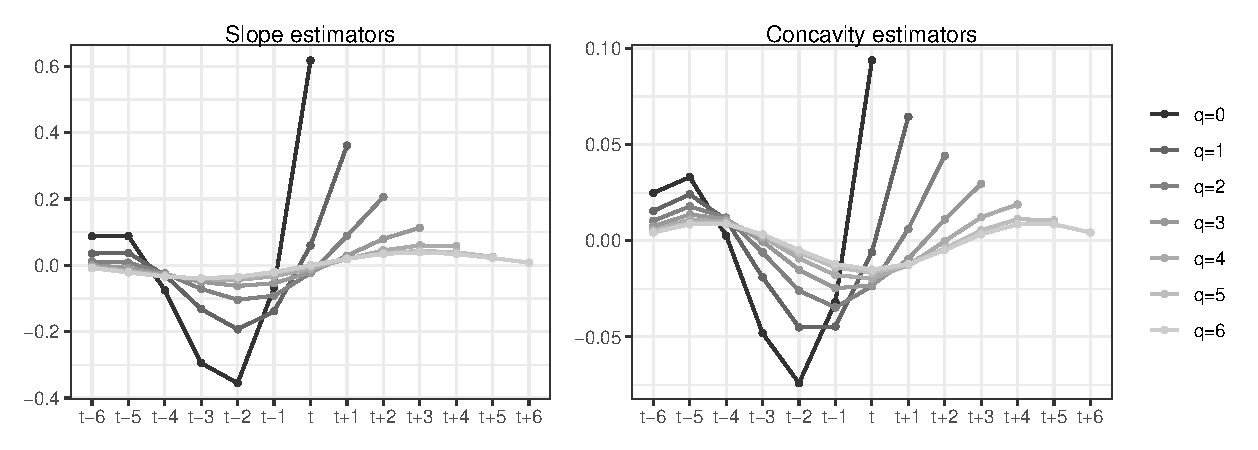
\includegraphics[width=0.9\textwidth,height=\textheight]{img/filters_used/mm_penteconcavite.pdf}

}

\end{figure}%

To distinguish the gain from the local parametrisation of the noise
associated to the real-time estimates of the slope and concavity, in the
empirical applications of section~\ref{sec-comparison} we also compares
the results to the final local parametrisation obtained by estimating
\(\delta\) using all the data (i.e., using the symmetric filters shown
in figure~\ref{fig-mmpenteconcac}), while maintaining a real-time
estimate of \(\sigma^2\). Figure~\ref{fig-mmpenteconcac-ex} shows an
example of the comparison of estimates of the ratio
\(|\delta_1/\sigma|\) with a global estimator (IC ratio) and two local
parametrisations:

\begin{itemize}
\item
  figure~\ref{fig-mmpenteconcac-ex-1}: using a symmetric filter to
  estimate \(\delta_1\) (final local parametrisation).
\item
  figure~\ref{fig-mmpenteconcac-ex-2}: using the asymmetric filter which
  need two points in the future to estimate \(\delta_1\). This is closed
  to the real-time estimates since two points in the future are needed
  to detect a turning point.
\end{itemize}

The turning points are clearly detected by the local estimators (slope
tends towards zero) when \(|\delta_1/\sigma|\) is estimated in the
real-time. However, the real-time local estimates of
\(|\delta_1/\sigma|\) are noisy: the variability of these estimates,
used to build asymmetric filters, will then lead to another source of
revisions in the intermediate estimates.

\begin{figure}[H]

\caption{\label{fig-mmpenteconcac-ex}Comparison of the estimates of
\(|\delta_1/\sigma|\) with a local estimator and global estimator (with
IC ratio) on a simulated series, the vertical lines being the simulated
turning points.}

\begin{minipage}{\linewidth}

\subcaption{\label{fig-mmpenteconcac-ex-1}Symmetric moving average used
for \(\hat \delta_1\).}

\centering{

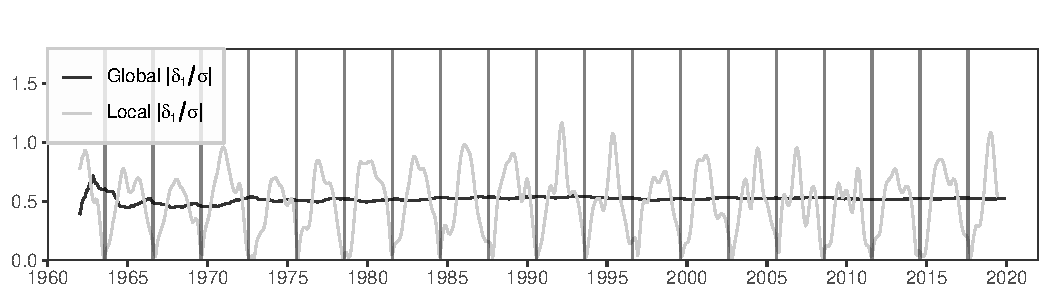
\includegraphics[width=0.9\textwidth,height=\textheight]{img/filters_used/mm_penteconcavite_ex.pdf}

}

\end{minipage}%
\newline
\begin{minipage}{\linewidth}

\subcaption{\label{fig-mmpenteconcac-ex-2}Asymmetric moving average
using two future points (\(q=2\)) used for \(\hat \delta_1\).}

\centering{

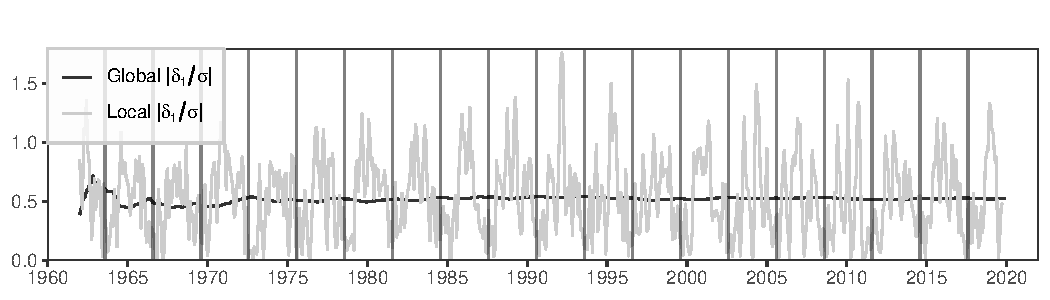
\includegraphics[width=0.9\textwidth,height=\textheight]{img/filters_used/mm_penteconcavite_ex2.pdf}

}

\end{minipage}%

\end{figure}%

There is no function in \texttt{rjd3filters} to directly compute those
moving averages but they can be easily computed using matrix computation
formula and applied to the series using \texttt{rjd3filters}.

\section{Comparison of different methods}\label{sec-comparison}

The different methods are compared on simulated and real data. For all
series, a symmetric 13-term filter is used: we then assume than the
bandwidth is fixed, as in the seasonal adjustment method X-11. A nearest
neighbour bandwidth is also tested (13-term asymmetric filters:
real-time filter uses observations between \(y_{t-12}\) and \(y_{t}\),
the second asymmetric filters uses observations between \(y_{t-11}\) and
\(y_{t+1}\), etc.) but with no improvement in the results (see
supplemental material). More complex methods to locally select
bandwidth, like the one proposed by \textcite{fan1992variable}, were not
tested. All the methods to create asymmetric filters are also compared
with estimates obtained by extending the series with an ARIMA model,
then applying a 13-term symmetric Henderson filter. The ARIMA model is
determined automatically, using \textcite{autoarima} algorithm (function
\texttt{forecast::auto.arima()}) on the last 12 years, with no seasonal
lag (the series being seasonally adjusted) and no external variables
(such as external regressors for correction of atypical points). The
performance of the different methods is judged on criteria relating to
revisions (between two consecutive estimates and in relation to the
final estimate) and the number of periods required to detect turning
points.

\subsection{Simulated series}\label{simulated-series}

\subsubsection{Methodology}\label{methodology}

Following a methodology close to that of \textcite{DarneDagum2009}, nine
monthly series are simulated between January 1960 and December 2020 with
different levels of variability. Each simulated series
\(y_t= C_t+ T_t + I_t\) can be written as the sum of three components:

\begin{itemize}
\item
  the cycle
  \(C_t = \rho [\cos (2 \pi t / \lambda) +\sin (2 \pi t / \lambda)]\),
  \(\lambda\) is fixed at 72 (6-year cycles, so there are 19 detectable
  turning points);
\item
  the trend \(T_t = T_{t-1} + \nu_t\) with
  \(\nu_t \sim \mathcal{N}(0, \sigma_\nu^2)\), \(\sigma_\nu\) being
  fixed at \(0.08\);
\item
  and the irregular \(I_t = e_t\) with
  \(e_t \sim \mathcal{N}(0, \sigma_e^2)\).
\end{itemize}

For the different simulations, we vary the parameters \(\rho\) and
\(\sigma_e^2\) in order to obtain series with different signal-to-noise
ratios (see figure~\ref{fig-graphs-data-simul}):

\begin{itemize}
\item
  High signal-to-noise ratio (i.e., low I-C ratio and low variability):
  \(\sigma_e^2=0.2\) and \(\rho = 3.0, 3.5\) or \(4.0\) (I-C ratio
  between 0.9 and 0.7);
\item
  Medium signal-to-noise ratio (i.e., medium I-C ratio and medium
  variability): \(\sigma_e^2=0.3\) and \(\rho = 1.5,\, 2.0\) or \(3.0\)
  (I-C ratio between 2.3 and 1.4);
\item
  Low signal-to-noise ratio (i.e., high I-C ratio and high variability):
  \(\sigma_e^2=0.4\) and \(\rho = 0.5,\, 0.7\) or \(1.0\) (I-C ratio
  between 8.9 and 5.2).
\end{itemize}

\begin{figure}[H]

\caption{\label{fig-graphs-data-simul}Simulated series with low
(\(\sigma_e^2=0.2\) and \(\rho = 3.55\)), medium (\(\sigma_e^2=0.3\) and
\(\rho = 2.0\)) and high variability (\(\sigma_e^2=0.4\) and
\(\rho = 1.0\)).}

\centering{

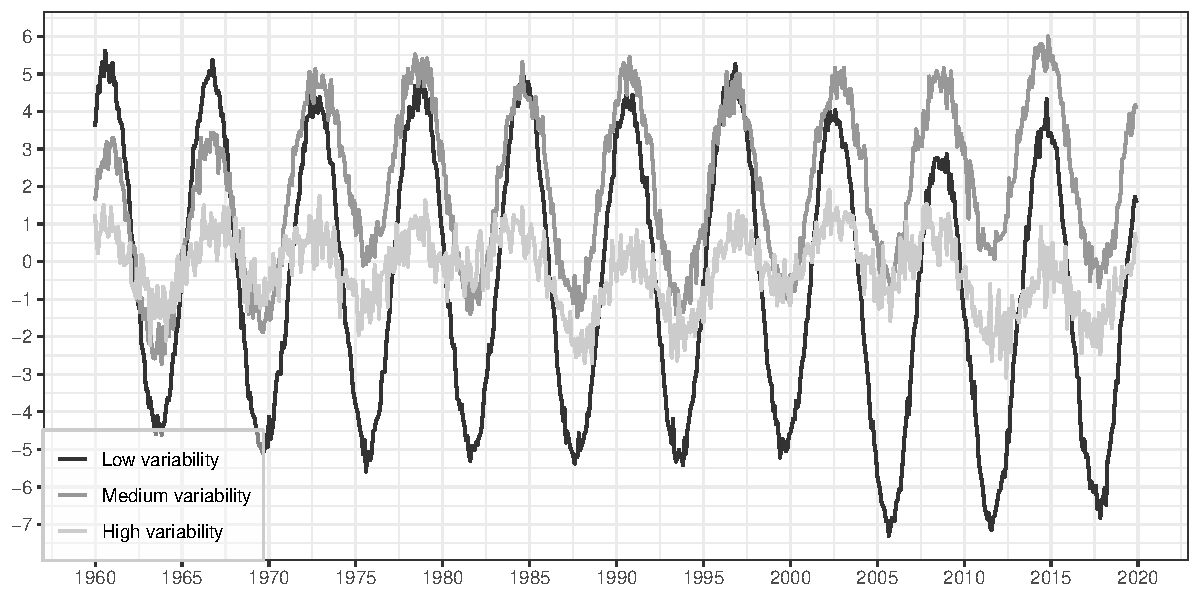
\includegraphics[width=1\textwidth,height=\textheight]{img/simulations/simul_data.pdf}

}

\end{figure}%

For each series and each date, the trend-cycle is estimated using the
different methods presented in this paper Three quality criteria are
computed:

\begin{enumerate}
\def\labelenumi{\arabic{enumi}.}
\item
  The \emph{phase shift} in the detection of turning points. In this
  paper, we focus on turning points associated to business cycle: it is
  defined as the succession of phases of economic recession and
  expansion, delimited by peaks (highest level of activity) and troughs
  (lowest level of activity), see for example \textcite{ferrara} for a
  description of the different economic cycles. In this paper, following
  \textcite{Zellner1991}, we used an accepted definition for
  turning-points:

  \begin{itemize}
  \tightlist
  \item
    An upturn occurs when the economy moves from a phase of recession to
    a phase of expansion. This is the case at date \(t\) when
    \(TC_{t-3}\geq TC_{t-2}\geq TC_{t-1}<TC_t\leq TC_{t+1}\).\\
  \item
    A downturn occurs when the economy moves from a phase of expansion
    to a phase of recession. This is the case at date \(t\) when
    \(TC_{t-3}\leq TC_{t-2}\leq TC_{t-1}>TC_t\geq TC_{t+1}\).
  \end{itemize}

  Let's denote \(TC_{t|t'}\) the estimate of the trend-cycle at date
  \(t\) using the data up to date \(t'\). The phase shift is often
  defined as the number of months required to detect the right turning
  point: it would then be equal to two if, in the case of a downturn,
  \(TC_{t-3|t+1}\leq TC_{t-2|t+1}\leq TC_{t-1|t+1}>TC_{t|t+1}\geq TC_{t+1|t+1}\)
  (two observations, at dates \(t\) and \(t+1\), are needed to qualify
  the date \(t\) as turning point). Note that, in that case, the phase
  shift could be equivalently set to 1 (only one observation after \(t\)
  is needed to define \(t\) as a turning point), without any difference
  on the comparison of the different methods.\\
  In this paper we use a slightly modified criterion: the \emph{phase
  shift} is defined as the number of months needed to detect the right
  turning point without any future revision. Thus, in the case of a
  downturn, the phase shift is two if
  \(TC_{t-3|t+1}\leq TC_{t-2|t+1}\leq TC_{t-1|t+1}>TC_{t|t+1}\geq TC_{t+1|t+1}\)
  and, for all dates \(t'\) higher than \(t+1\):
  \(TC_{t-3|t'}\leq TC_{t-2|t'}\leq TC_{t-1|t'}>TC_{t|t'}\geq TC_{t+1|t'}\).
  Since a 13-term Henderson filter is used for the final estimates of
  the trend-cycle, the phase shift is at most height (the final estimate
  of \(TC_{t+1}\) is compute at the date \(t+7\)). This definition is
  used because it can happen that the right turning point is detected by
  asymmetric filters but is not detected by the final estimate using a
  symmetric filter (this is the case for 41 reversal points out of the 9
  series with asymmetric Musgrave filters) or that there are revisions
  in successive estimates (this is the case for 7 turning points out of
  the 9 series with asymmetric Musgrave filters). Finally, relatively
  few turning points are detected at the right date with the final
  estimate. With the 13-term Henderson filter, 18 are correctly detected
  in series with low variability (out of 57 possible), 11 in series with
  medium variability and 12 in series with high variability.
\item
  The average of the relative deviations between to the last estimate
  (comparison of the \(q\)\textsuperscript{th} estimate and the last
  estimate): \[
  MAE_{fe}(q)=\mathbb E\left[
  \left|\frac{
  TC_{t|t+q} -  TC_{t|last}
  }{
   TC_{t|last}
  }\right|
  \right].
  \]
\item
  The average of the relative deviations between two consecutive
  estimates (the \(q\)\textsuperscript{th} estimate and the
  \(q+1\)\textsuperscript{th} estimate): \[
  MAE_{ce}(q)=\mathbb E\left[
  \left|\frac{
  TC_{t|t+q} - TC_{t|t+q+1}
  }{
  TC_{t|t+q+1}
  }\right|
  \right].
  \]
\end{enumerate}

The simulated series are of length 60 years, which is often not
realistic for economic time series. However, since all the methods are
local, the results are not affected by the length of the series. The
length of the series would only have an impact for the identification
and the estimation of the ARIMA model. In this case, since the same data
generating process is used during the 60 years, it could be relevant to
identify the ARIMA model using all the data. Even if it would improve
the results in term of phase shift (see supplemental material) we prefer
to only use the last 12 years to identify and estimate the ARIMA model,
to be closer to what would have been done with a real-time series.

\subsection{Comparison}\label{comparison}

Excluding for the moment the local parametrisations of the polynomial
filters, the linear-constant polynomial filter (LC) seems to give the
best results in terms of delay in the detection of turning points
(figure~\ref{fig-graphstpsimul}). Performance is relatively close to
that obtained by extending the series using an ARIMA model. However,
when variability is low, the LC filter seems to give poorer results and
the quadratic-linear polynomial filter (QL) seems to give the best
results.

For series with moderate variability, local parametrisation of the LC
and QL filters reduces the phase shift. For series with high
variability, the phase shift is only reduced by using the final
\(\hat\delta\) parameters: real-time estimates seem to add more
variance. For series with low variability, performance seems to be
slightly improved only with the LC filter.

\begin{figure}[H]

\caption{\label{fig-graphstpsimul}Distribution of phase shift on
simulated series.}

\centering{

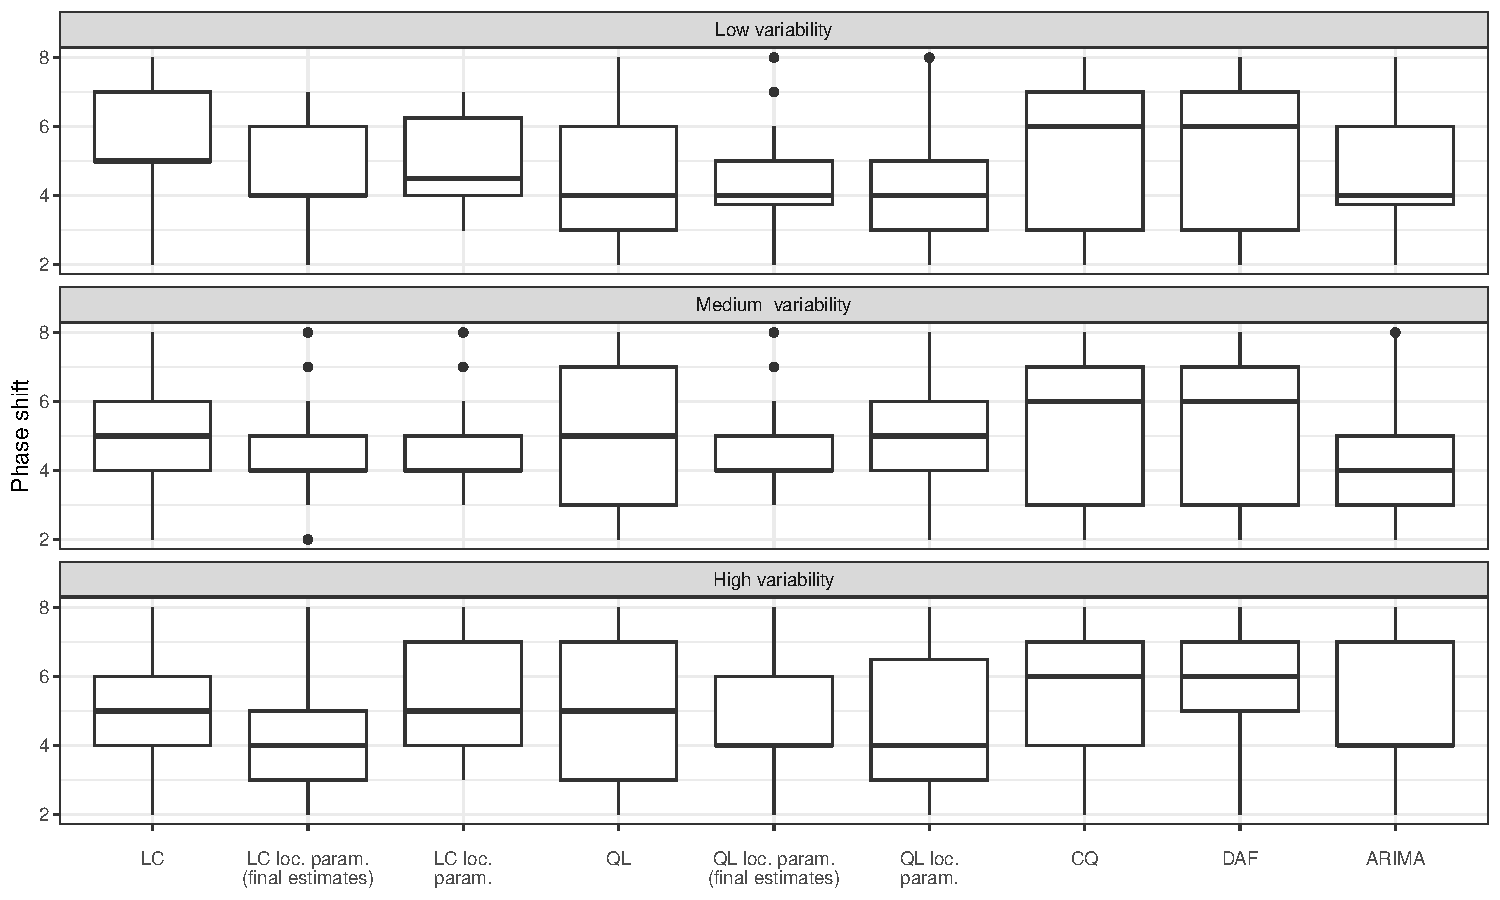
\includegraphics[width=1\textwidth,height=\textheight]{img/simulations/phase_shift_simul.pdf}

\justifying

\emph{Lecture: this plots represent box plots of the phase shift: the
box represents the interquartile range, the central horizontal line the
median the dot the outliers and the whisker the range of the data (if no
outlier).}\\
\emph{For simulated series with medium variability (when a symmetric
filter of length 13 is relevant), with the linear constant (LC) method,
50\% of the turning point are detected with a phase shift of at most 5
months whereas when the LC filter is parametrised locally, 50\% of the
turning point are detected with a phase shift of at most 4 months.}
\emph{For the direct asymmetric filter (DAF), 25\% of the turning are
detected with a phase shift of at least 7 months (compares to 5 for the
LC method).}

}

\end{figure}%

In terms of revisions, the variability of the series has little effect
on the respective performances of the different methods, but it does
affect the orders of magnitude, which is why the results are presented
only for series with medium variability (table~\ref{tbl-simulrev}). In
general, LC filters always minimise revisions (with relatively small
effect from the local parametrisation of the filters) and revisions are
greater with cubic-quadratic (CQ) and direct (DAF) polynomial filters.

For the QL filter, there is a large revision between the second and
third estimates: this may be due to the fact that for the second
estimate (when one point in the future is known), the QL filter assigns
a greater weight to the estimate in \(t+1\) than to the estimate in
\(t\), which creates a discontinuity. This revision is considerably
reduced by parametrising the filter locally. For polynomial filters
other than the LC filter, the large revisions at the first estimate were
to be expected given the coefficient curve: a very large weight is
associated with the current observation and there is a strong
discontinuity between the moving average used for real-time estimation
(when no point in the future is known) and the other moving averages.

Extending the series using an ARIMA model gives revisions with the
latest estimates of the same order of magnitude as the LC filter, but
slightly larger revisions between consecutive estimates, particularly
between the fourth and fifth estimates (as might be expected as
highlighted in section~\ref{sec-mmasym}).

\begin{table}

\caption{\label{tbl-simulrev}Average of the relative deviations of the
revisions for the different filters on simulated series with medium
variability.}

\centering{

\begin{tabular}{ccccccc}
\toprule
Method & $q=0$ & $q=1$ & $q=2$ & $q=3$ & $q=4$ & $q=5$\\
\midrule
\addlinespace[0.3em]
\multicolumn{7}{l}{\textbf{$MAE_{fe}(q) = \mathbb E\left[\left|(TC_{t|t+q} -  TC_{t|last})/TC_{t|last}\right|\right]$}}\\
\hspace{1em}LC & 0.21 & 0.10 & 0.03 & 0.03 & 0.03 & 0.01\\
\hspace{1em}LC local param. (final estimates) & 0.19 & 0.09 & 0.03 & 0.03 & 0.03 & 0.01\\
\hspace{1em}LC local param. & 0.29 & 0.10 & 0.03 & 0.03 & 0.03 & 0.01\\
\hspace{1em}QL & 0.33 & 0.10 & 0.04 & 0.04 & 0.03 & 0.01\\
\hspace{1em}QL local param. (final estimates) & 0.21 & 0.10 & 0.03 & 0.03 & 0.03 & 0.01\\
\hspace{1em}QL local param. & 0.30 & 0.10 & 0.04 & 0.03 & 0.03 & 0.01\\
\hspace{1em}CQ & 0.45 & 0.13 & 0.13 & 0.09 & 0.06 & 0.02\\
\hspace{1em}DAF & 0.47 & 0.15 & 0.15 & 0.09 & 0.06 & 0.02\\
\hspace{1em}ARIMA & 0.22 & 0.10 & 0.03 & 0.03 & 0.03 & 0.01\\
\addlinespace[0.3em]
\multicolumn{7}{l}{\textbf{$MAE_{ce}(q)=\mathbb E\left[
\left|(TC_{t|t+q} - TC_{t|t+q+1})/TC_{t|t+q+1}\right|
\right]$}}\\
\hspace{1em}LC & 0.19 & 0.10 & 0.02 & 0.01 & 0.07 & 0.01\\
\hspace{1em}LC local param. (final estimates) & 0.20 & 0.10 & 0.03 & 0.01 & 0.05 & 0.01\\
\hspace{1em}LC local param. & 0.24 & 0.11 & 0.03 & 0.01 & 0.05 & 0.01\\
\hspace{1em}QL & 0.29 & 3.46 & 0.00 & 0.03 & 0.04 & 0.01\\
\hspace{1em}QL local param. (final estimates) & 0.31 & 0.11 & 0.02 & 0.01 & 0.04 & 0.01\\
\hspace{1em}QL local param. & 0.24 & 0.16 & 0.00 & 0.03 & 0.04 & 0.01\\
\hspace{1em}CQ & 0.43 & 0.02 & 0.10 & 0.07 & 0.05 & 0.02\\
\hspace{1em}DAF & 0.66 & 0.24 & 0.11 & 0.14 & 0.06 & 0.02\\
\hspace{1em}ARIMA & 0.23 & 0.10 & 0.02 & 0.03 & 0.25 & 0.01\\
\bottomrule
\end{tabular}

\justifying

\emph{Lecture: the estimates for \(q=0\) correspond to the first
estimates of the trend-cycle (real-time estimates when 0 point in the
future is known), \(q=1\) correspond to the second estimates of the
trend-cycle (when 1 point in the future is known).} \emph{Since the
final estimates are obtain using a symmetric filter of bandwidth 6,
\(q=6\) corresponds to the final estimates of the trend-cycle (when 6
points in the future are known).} \emph{\(MAE_{fe}(0)\) compares the
revision between the first estimate (\(q=0\)) and the last estimate
(\(q=6\)) and \(MAE_{ce}(0)\) compares the revision between the first
estimate (\(q=0\)) and the second estimate (\(q=1\)).}

}

\end{table}%

\subsection{Real series}\label{real-series}

The differences between the methods are also illustrated using an
example from the FRED-MD database (\textcite{fredmd}) containing
economic series on the United States. This database facilitates the
reproducibility of the results thanks to the availability of series
published on past dates. The series studied correspond to the database
published in November 2022. It is the level of employment in the United
States (series \texttt{CE160V}, used in logarithm) around the February
2001 turning point, consistent with the monthly dating of the turning
points. This turning point was chosen because it is particularly visible
in the raw series (figure~\ref{fig-ce16ov-previmp-lp}) and this series
was select because it is used for dating economic cycles. Studying the
series up to January 2020, this series has a medium variability: a
symmetric filter of 13 terms is therefore appropriate.

Figure~\ref{fig-ce16ovlp} shows the successive estimates of the
trend-cycle using the different methods studied. For this series, the
phase shift is 6 months for the LC and CQ methods and the extension of
the series by ARIMA. It is of two months for the other methods (QL,
DAF). In this example, local parametrisation does not reduce the phase
shift, but it does reduce revisions. The QL and DAF polynomials lead to
greater variability in the intermediate estimates, especially in
February 2001.

\begin{figure}[H]

\caption{\label{fig-ce16ovlp}Successive estimates of the trend-cycle in
US employment (in logarithms).}

\centering{

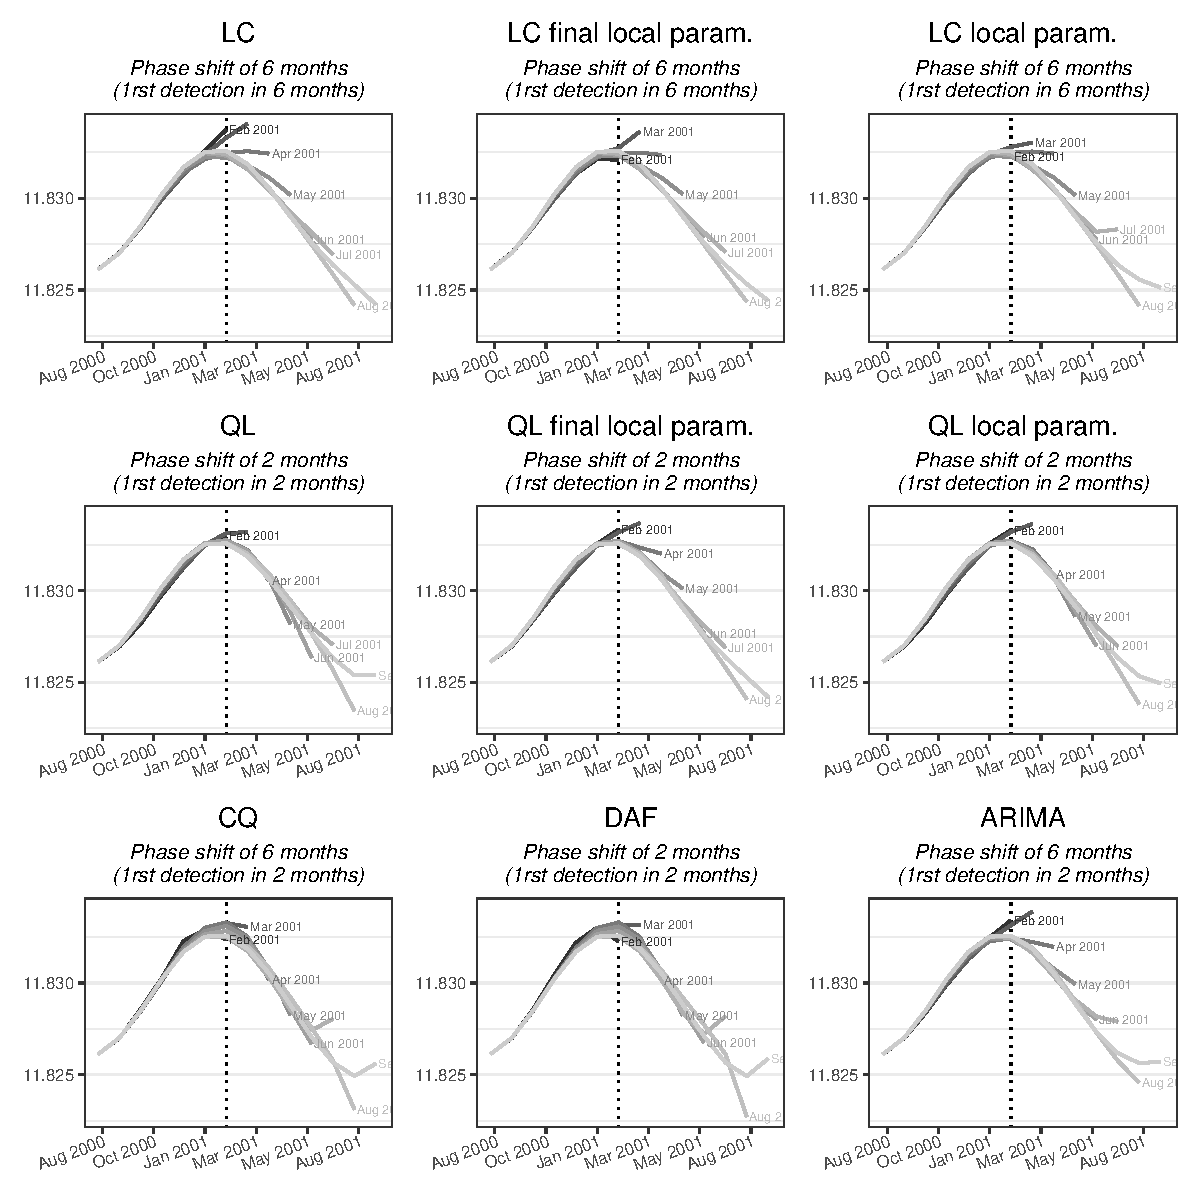
\includegraphics[width=0.95\textwidth,height=\textheight]{img/nber/ce16ov_fev2001_lp.pdf}

\justifying

\emph{Lecture: the dotted vertical line corresponds to the date of the
turning point (February 2001).} \emph{The curve ``Feb 2001'' corresponds
to the estimates of the trend-cycle using the data observed until
February 2001.} \emph{Since a 13-term Henderson filter is used for the
final estimates, for the curve ``Feb 2001'' estimates from September
2001 to February 2001 are intermediate estimates.}

}

\end{figure}%

The quality of the intermediate estimates can also be analysed using the
implicit forecasts of the different methods
(figure~\ref{fig-ce16ov-previmp-lp}). As a reminder, these are forecasts
of the raw series which, by applying the symmetric Henderson filter to
the extended series, give the same estimates as the asymmetric moving
averages. The forecasts of the ARIMA model are naive and do not take the
turning point into account, unlike the other methods. Finally, local
parametrisation of the QL filter produces much more consistent
forecasts.

\begin{figure}[H]

\caption{\label{fig-ce16ov-previmp-lp}Implicit forecasts linked to
successive estimates of the trend-cycle in US employment (in logarithms)
using local polynomial methods.}

\centering{

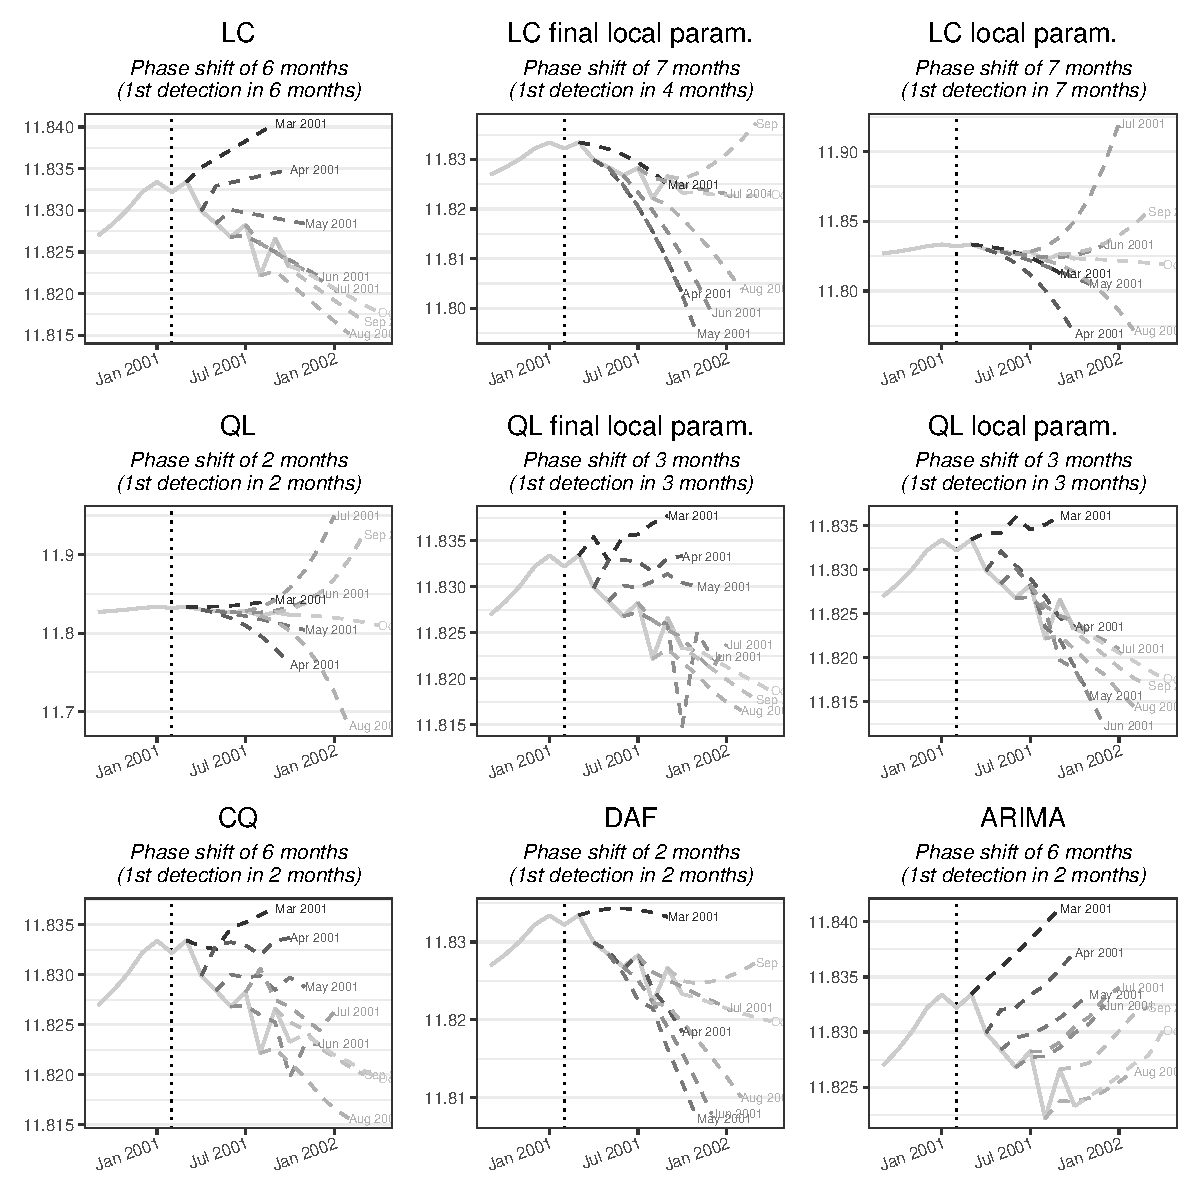
\includegraphics[width=0.95\textwidth,height=\textheight]{img/nber/ce16ov_fev2001_prev_imp_lp.pdf}

\justifying

\emph{Lecture: the dotted vertical line corresponds to the date of the
turning point (February 2001).} \emph{The curve ``Mar 2001'' corresponds
to the implicit forecasts associated to the asymmetric filters used for
the trend-cycle estimations using the data observed until March 2001.}

}

\end{figure}%

\subsection{Discussion}\label{discussion}

In the section we discuss the applicability of the presented methods to
other frequencies (section~\ref{sec-other-freq}) and some limits of the
presented methods (for example sensitivity to outliers like COVID-19,
section~\ref{sec-out-covid}) .

\subsubsection{Other frequencies}\label{sec-other-freq}

In this paper, we focused on monthly series, but the methods presented
can be applied to other frequencies. In general, for lower frequencies,
the bandwidth of the symmetric filter reduced. For example, for
quarterly series, X-11 uses a 5-term symmetric filter (in general) or
7-term symmetric filter for series with high variability. Mechanically,
since fewer points are used, there will be less differences between
methods in term of phase shift. For example, on simulated series the
results are similar in terms of phase shift but revisions are reduced
with local parametrisation (see supplemental material).

Since X-13ARIMA-SEATS can only be applied for series with frequency
lower than monthly, for higher frequencies (weekly, daily, etc.), there
is no reference on the length of the filters to uses. The length of the
filters can be determined using local polynomial methods, for example
minimising a cross-validation statistics (using the function
\texttt{rjd3filters::cross\_validation()}) or with more complex methods
as describe by \textcite{Loader1999}, but it will surely be necessary to
use higher bandwidth than for monthly series. The larger the window, the
greater the bias in assuming that the trend is locally of degree 1: the
LC method will then be certainly less appropriate than other methods
(QL, CQ or DAF). Moreover, since the bias is higher, the local
parametrisation of the filters will surely have more impact.

\subsubsection{Outliers and COVID-19}\label{sec-out-covid}

In this article and in those associated to trend-cycle extraction
techniques, the moving averages are applied and compared on series
already seasonally adjusted or without seasonality (simulated series).
The revisions and the phase shift are limited to 8 months (when the
symmetric filter is 13 terms) and this has the advantage of isolating
the impacts of the different filters from the other processes inherent
in seasonal adjustment. There are, however, two drawbacks to this
simplification:

\begin{enumerate}
\def\labelenumi{\arabic{enumi}.}
\item
  The estimation of the seasonally-adjusted series depends on the method
  used to extract the trend-cycle. The choice of method used to estimate
  the trend-cycle can therefore have an impact well beyond 6 months
  (when a 13-term Henderson filter is used).
\item
  As moving averages are linear operators, they are sensitive to the
  presence of atypical points. Direct application of the methods can
  therefore lead to biased estimates, due to their presence, whereas
  seasonal adjustment methods (such as the X-13ARIMA-SEATS method) have
  a correction module for atypical points. Furthermore, as shown in
  particular by \textcite{dagum1996new}, the final symmetric filter used
  by X-13ARIMA-SEATS to extract the trend-cycle (and therefore the one
  indirectly used when applying the methods to seasonally-adjusted
  series), reduces by just 38\% cycles of length 9 and 10 months
  (generally associated with noise rather than the trend-cycle). The
  final asymmetric filters even amplify 9 and 10-month cycles. This can
  result in the introduction of undesirable ripples, i.e., the detection
  of false turning points. This problem is reduced by correcting
  atypical points and the \emph{Nonlinear Dagum Filter} (NLDF) was
  defined in this perspective:

  \begin{enumerate}
  \def\labelenumii{\alph{enumii}.}
  \item
    applying the X-11 atypical point correction algorithm \autocite[see
    for example][ for a description]{ladiray2011seasonal} to the
    seasonally adjusted series, then extending it with an ARIMA model;
  \item
    perform a new atypical point correction using a much stricter
    threshold and then apply the 13-term symmetric filter. Assuming a
    normal distribution, this amounts to modifying 48\% of the irregular
    values.
  \end{enumerate}

  The \emph{cascade linear filter} (CLF), studied in particular in
  \textcite{dagumBianconcini2023}, corresponds to an approximation of
  the NLDF using a 13-term filter and when the forecasts are obtained
  from an ARIMA(0,1,1) model where \(\theta=0.40.\).
\end{enumerate}

Figure~\ref{fig-ce16ovcovid} and figure~\ref{fig-ce16ov-previmp-covid}
show the successive estimates of the trend-cycle and the associated
implicit forecast for the US employment during the COVID-19. First, we
observe that while the real turning point is in April 2020, the 13-term
Henderson filter produces final estimates of the trend-cycles, biased by
the presence of a huge outlier, which lead to a turning point detected
in June 2020. Second, as in 2001, the CQ and DAF methods lead to lots of
variability in the intermediate estimates. For the QL method, the local
parametrisation seems to slightly reduce the revisions. For the LC
method, local parametrisation has few impact on the estimates of the
trend-cycle but the associated implicit forecasts are not plausible: the
final estimate of the slope is biased by the outlier. Third, the ARIMA
model can lead to unrealistic forecasts.

\begin{figure}[H]

\caption{\label{fig-ce16ovcovid}Successive estimates of the trend-cycle
in US employment (in logarithms) during the COVID-19.}

\centering{

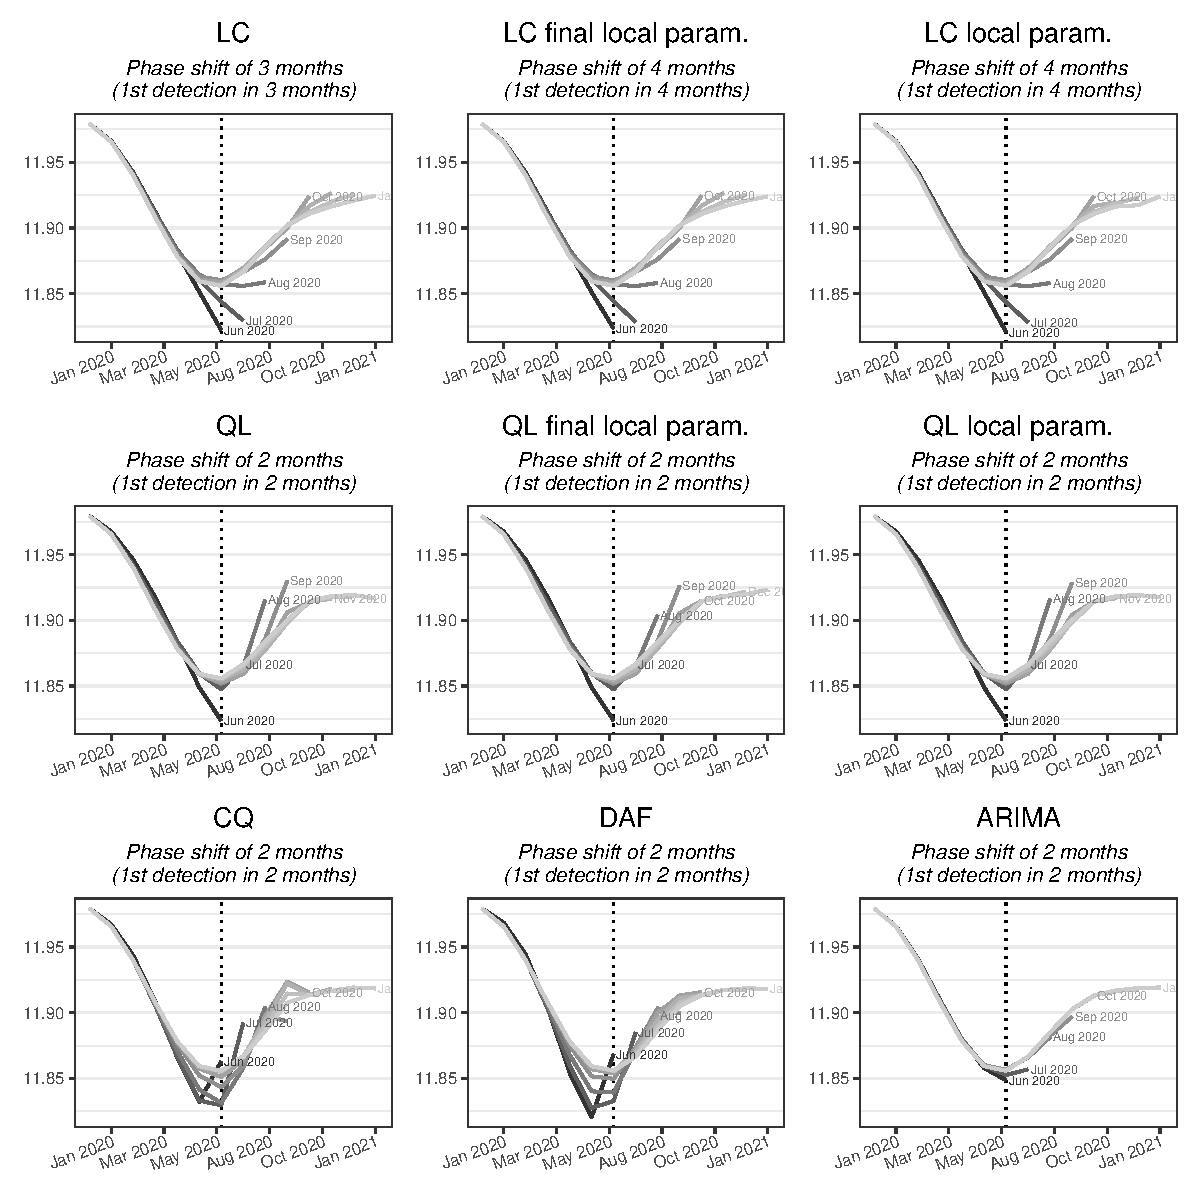
\includegraphics[width=0.95\textwidth,height=\textheight]{img/nber/ce16ov_covid_lp.pdf}

\justifying

\emph{Lecture: the dotted vertical line corresponds to the date of the
turning point (June 2020) detected with the 13-term Henderson filter but
the real one is June 2020.} \emph{The curve ``Apr 2020'' corresponds to
the estimates of the trend-cycle using the data observed until April
2020.}

}

\end{figure}%

\begin{figure}[H]

\caption{\label{fig-ce16ov-previmp-covid}Implicit forecasts linked to
successive estimates of the trend-cycle in US employment (in logarithms)
using local polynomial methods during the COVID-19.}

\centering{

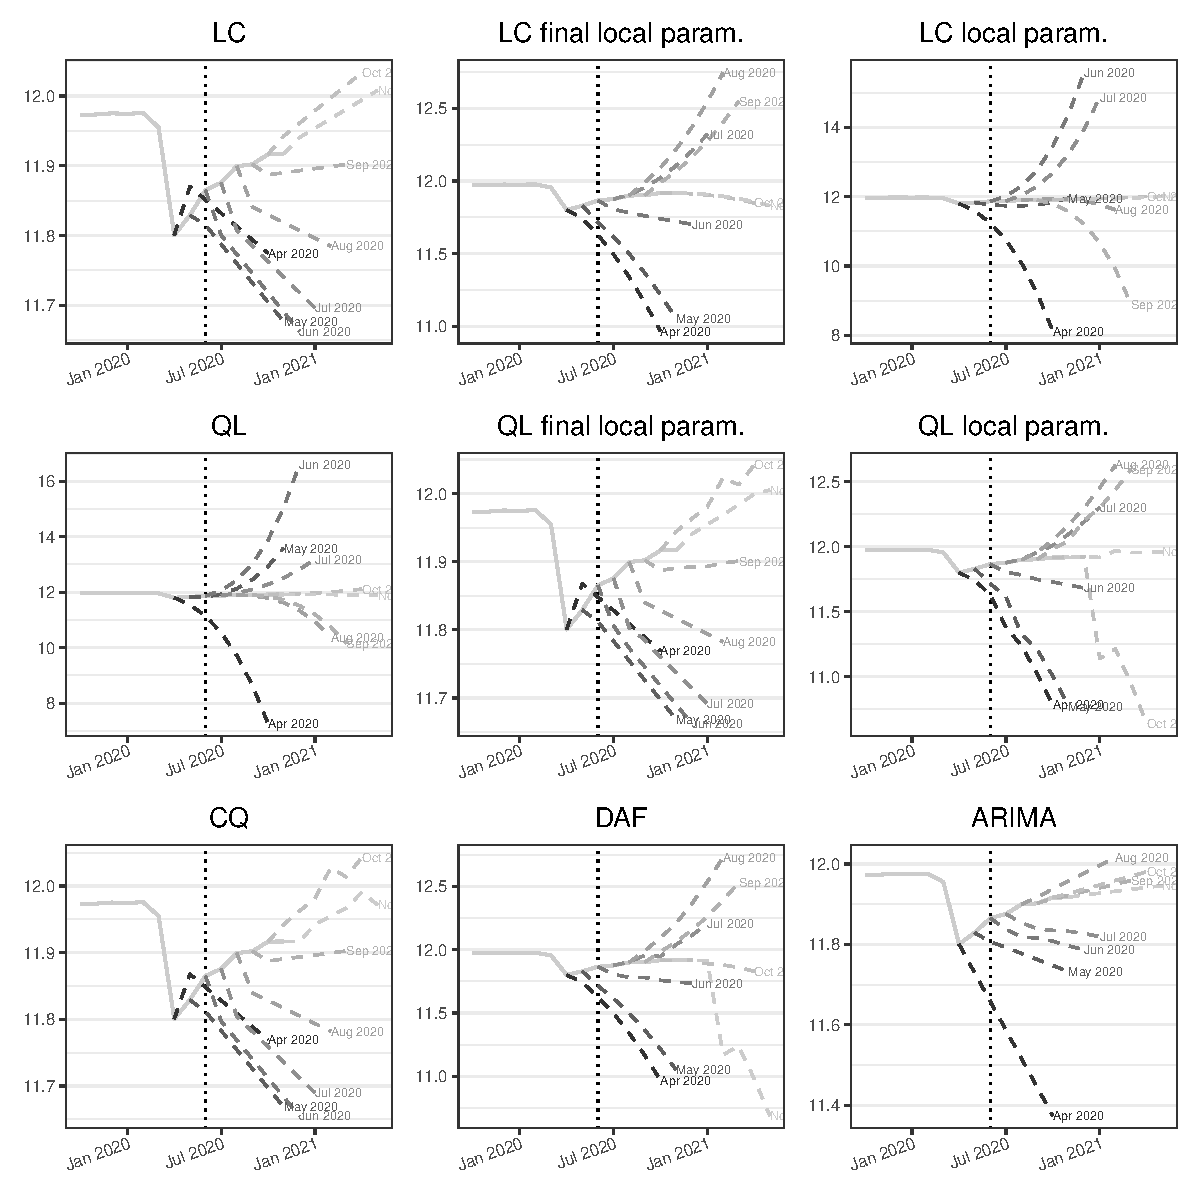
\includegraphics[width=0.95\textwidth,height=\textheight]{img/nber/ce16ov_covid_prev_imp_lp.pdf}

\justifying

\emph{Lecture: the curve ``Apr 2020'' corresponds to the implicit
forecasts associated to the asymmetric filters used for the trend-cycle
estimations using the data observed until April 2020.}

}

\end{figure}%

To sum up, trend-cycle estimates are biased by the presence of outliers
which can also impact the detection of turning-points. Several approach
could be used to limit their impact of to directly take them into
account:

\begin{itemize}
\item
  Adjustment of outliers prior to filtering, for example with a RegARIMA
  model or other correction modules like the one used in X-11.
\item
  Increase the bandwidth of the filter used to extract the trend-cycle
  (it will smooth the trend-cycle by giving less weights to the atypical
  points).
\item
  Since all the filter studied in this paper are equivalent to a local
  polynomial model, an external regressor can be added to the linear
  model to handle the outlier (the matrix \(\boldsymbol X\) would then
  be modified). In the case of an additive outlier, this is equivalent
  to set to 0 the coefficient of the moving average associated to the
  date of the outlier (using \(y_{t-h}\) to \(y_{t+h}\) for the
  trend-cycle estimates, if the outlier is at the date \(t\) the central
  coefficient is set to 0) and renormalise the sum of the coefficients
  to 1.
\item
  Use of robust methods to estimate the trend-cycle, such as robust
  local regressions or moving medians.
\end{itemize}

\section{Conclusion}\label{conclusion}

For business cycle analysis, most statisticians use trend-cycle
extraction methods, either directly or indirectly. They are used, for
example, to reduce the noise of an indicator in order to improve its
analysis, and models, such as forecasting models, usually use seasonally
adjusted series based on these methods.

This paper presents the R package \texttt{rjd3filters}, which implements
several methods to build moving averages for real-time trend-cycle
estimation. It also offers various functions for the theoretical
analysis of moving averages (gain functions, phase shift, quality
criteria, etc.) and judging the quality of the latest estimates (for
example with implicit forecasts). It also makes it easy to combine
moving averages and also to integrate custom moving averages into the
X-11 seasonal adjustment algorithm (with the
\texttt{rjd3filters::x11plus\_trend()} function). \texttt{rjd3filters}
thus facilitates research into the use of moving averages as part of
real-time cycle trend estimation. This is the case, for example, with
the local parametrisation of Musgrave moving averages and other
asymmetric moving averages linked to local polynomial regression,
presented in this article.

By comparing the different methods, we can learn a few lessons about the
construction of these moving averages.\\
During economic downturns, asymmetric filters used as an alternative to
extending the series using the ARIMA model can reduce revisions to
intermediate estimates of the trend-cycle and enable turning points to
be detected more quickly.\\
At the end of the period, modelling polynomial trends of degree greater
than three (cubic-quadratic, CQ, and direct, DAF) seems to introduce
variance into the estimates (and therefore more revisions) without
allowing faster detection of turning points. For real-time estimates of
the trend-cycle, we can therefore restrict ourselves to methods
modelling polynomial trends of degree two or less (linear-constant, LC,
and quadratic-linear, QL). In addition, parametrising polynomial filters
locally as proposed in this paper enables turning points to be detected
more quickly (especially for the QL filter). Even when the phase shift
is not reduced, local parametrisation is recommended because it reduces
revisions and produces intermediate estimates that are more consistent
with expected future trends. However, with these methods, the length of
the filter used must be adapted to the variability of the series: if the
filter used is too long (i.e., if the variability of the series is
``low''), retaining polynomial trends of degree one or less (LC method)
produces poorer results in terms of detecting turning points.

This study could be extended in many ways. One possible extension would
be to look at the impact of filter length on the detection of turning
points. Asymmetric filters are calibrated using indicators calculated
for the estimation of symmetric filters (for example, to automatically
determine their length), whereas a local estimate might be preferable.
Furthermore, we have only focused on monthly series with a 13-term
symmetric filter, but the results may be different if the symmetric
filter studied is longer or shorter and if we study series with other
frequencies (weekly or daily, for example).

Another possibility could be to study the impact of atypical points:
moving averages, like any linear operator, are highly sensitive to the
presence of atypical points. To limit their impact, in X-11 a strong
correction for atypical points is performed on the irregular component
before applying the filters to extract the trend-cycle. This leads to
examining the impact of these outliers on the estimation of the
trend-cycle and turning points, and also to explore new types of
asymmetric filters based on robust methods (such as robust local
regressions or moving medians).

\newpage

\section*{References}\label{references}
\addcontentsline{toc}{section}{References}

\printbibliography[heading=none]




\end{document}
